
\documentclass[a4paper]{article}
\usepackage[spanish]{babel}

\usepackage[backend=biber,
style=apa,
]{biblatex}

\newcommand\invisiblesection[1]{%
  \refstepcounter{section}%
  \addcontentsline{toc}{section}{\protect\numberline{\thesection}#1}%
  \sectionmark{#1}}

\defbibenvironment{bibliography}
  {\enumerate
     {}
     {\setlength{\leftmargin}{\bibhang}%
      \setlength{\itemindent}{-\leftmargin}%
      \setlength{\itemsep}{\bibitemsep}%
      \setlength{\parsep}{\bibparsep}}}
  {\endenumerate}
  {\item}


\usepackage{caption} % Para poner captions the multiples renglones
\usepackage{float} % Para colocar las imágenes
\usepackage{fullpage} % Package to use full page


\usepackage{parskip} % Package to tweak paragraph skipping
\usepackage{tikz} % Package for drawing
\usepackage{amsmath}
\usepackage{amssymb} % Para usar \mathbb
\usepackage{csquotes}

\usepackage{outlines} % Para enumerar con multiples niveles

\usepackage{graphicx} % Para instertar pdfs como imágenes y usar \scalebox

% Paraa induces:

\usepackage{imakeidx}
\makeindex[columns=3, title=Alphabetical Index, intoc]


\newcommand*{\Scale}[2][4]{\scalebox{#1}{$#2$}}%
\newcommand*{\Resize}[2]{\resizebox{#1}{!}{$#2$}}%

\usepackage{minted} % Para colocar código
\usemintedstyle{bw} % Para usar blanco y negro como colores de código

\renewcommand{\figurename}{Figura}
\renewcommand{\tablename}{Tabla}
\renewcommand\listingscaption{Listado}

\setlength{\parskip}{\baselineskip}%
\setlength{\parindent}{0pt}%


\addbibresource{bibliography.bib}
\begin{document}

\hspace{0pt}
\vfill

\invisiblesection{Portada}

\begin{center}
    {\huge Aplicación del Álgebra Lineal:\\Ofuscación binaria}\\    \quad\\
    {\large Universidad Panamericana}\\
    {\large Facultad de Ingeniería}\\
    \quad\\
    \quad\\
    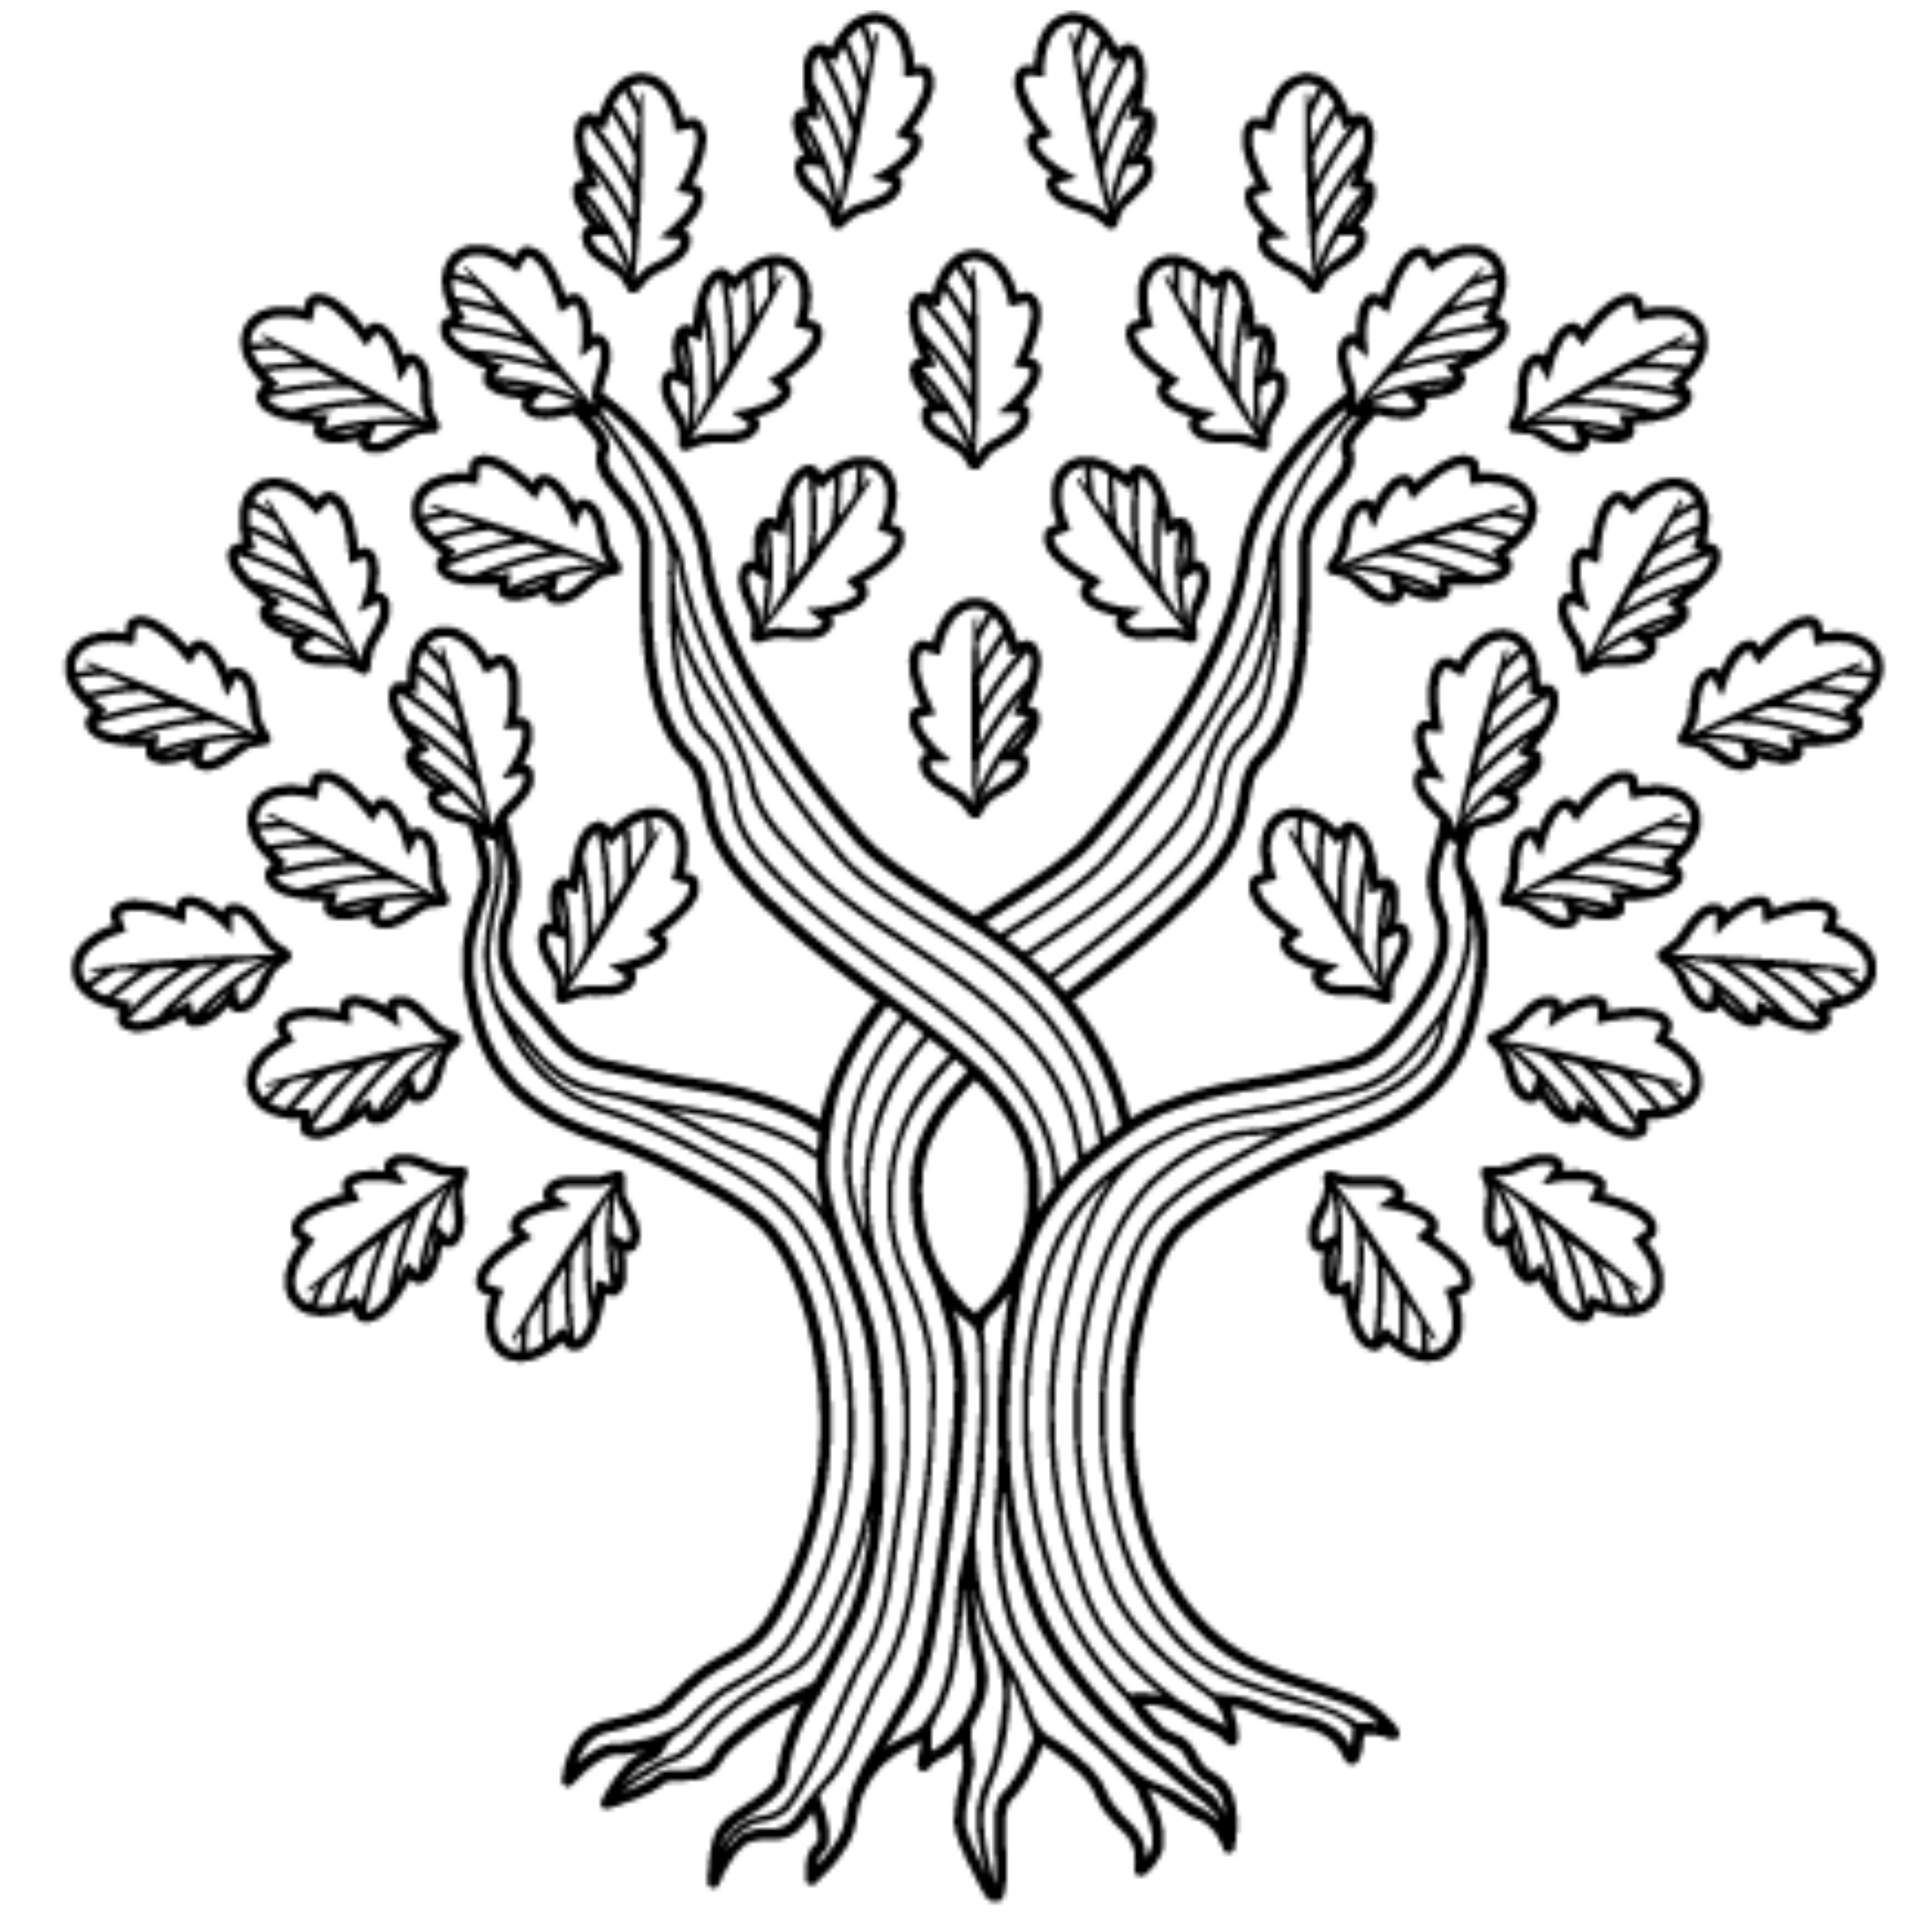
\includegraphics[scale=0.3]{UP}
    \quad\\
    \quad\\
    Álgebra Lineal\\
    Prof. Miguel Angel Quintero Zamarron\\
    \quad\\
    \quad\\
    \begin{tabular}{c|c}
        Díaz Barriga Rodrigo Peña & 0249221\\
        Osornio López Daniel Alejandro & 0244685\\
        Paredes García Ricardo & 0241528
    \end{tabular}\\
    \quad\\
    \quad\\
\end{center}

\vfill

\newpage
\tableofcontents

\newpage
\section{Objetivos}

1. Diseño de un algoritmo de cifrado que utilice como herramienta principal el
álgebra lineal

2. Creación de un ejecutable de ofuscación de archivos

\quad 2.1. Implementación de un script de cifrado de archivos con Mathematica

\quad 2.2. Implementación del algoritmo del punto 2.2 para desarrollar una herramienta de 
ofuscación
de
archivos
binarios
y
de
texto 

\quad 2.3. Verificación de ofuscación con herramientas de ingeniería inversa

\section{Resumen}

El objetivo de este proyecto es utilizar transformaciones lineales como llaves
para cifrar y descifrar bits de información.
Se explora el uso de la aritmética modular para mantener la congruencia de la
información
 a la vez que se experimenta con distintos métodos de cifrado por medio de
algoritmos varios que emplean las transformaciones en su proceso.
La meta es implementar una herramienta de cifrado y descifrado que pueda
proteger tanto archivos de texto como ejecutables con un procedimiento
que permita su auto descifrado junto con soporte a \textit{passphrases} para
obtener mayor seguridad.

Los métodos estudiados son dos. 

El primero es una modificación de un cifrado de sustitución. Primero se
construye una matriz que contiene todos los valores representables en un 
byte y modifica la matriz por medio de multiplicaciones matriciales para
después sustituir cada byte en el archivo por su nuevo valor. 

El segundo, ordena todos los bytes del mensaje a cifrar, como puede ser un
archivo, y le aplica una multiplicación matricial a la totalidad del archivo. 

Para dar soporte al auto-descifrado de los archivos, cuando se utilice la
bandera --auto, se almacenan en el archivo los valores para descifrarse a sí
mismo, 
con bytes de meta información que facilitan el proceso y permiten una mayor
seguridad lograda por el factor aleatorio. Este proyecto plantea la
implementación 
de una librería de cifrado de archivos por medio de una ofuscación binaria
lograda por transformaciones.

\newpage
\section{Introducción}

Como estudiantes de la carrera de Inteligencia de Datos y Ciberseguridad,
decidimos desarrollar el proyecto sobre un tema que permite darnos una noción
del funcionamiento de las computadoras al desarrollar un sistema que se
encargue de cifrar archivos de todo tipo, modificando los bytes del mismo por
los que una transformación lineal dicte.

Antes de empezar a programar nada, desarrollaremos el algoritmo de cifrado que
emplearemos; describiremos los conceptos
necesarios para llegar a dicho procedimiento y los patrones que contiene para
analizar si es posible su cifrado de forma sencilla.

Una vez tengamos listo el algoritmo, implementaremos un script de uso
general para el cifrado de arreglos de bytes utilizando el lenguaje de
programación Rust
\iffalse
Wolfram Mathematica. 

Decidimos emplearlo debido a la facilidad que tiene en su programación, manejo
de datos, de matrices
y la facilidad que tiene para interactuar con el sistema con una gran riqueza de
funciones matemáticas disponibles para obtener resultados con gran velocidad
además
de ofrecernos la realización de material gráfico agradable y sencillo de
reproducir
para ilustrar nuestra experimentación y resultados.
\fi

Decidimos emplearlo debido a la facilidad que tiene en su
sintaxis sumada con las operaciones de bajo nivel que permite realizar con la
computadora sin necesidad de producir código complejo como pasaría con
C/C++.

Verificaremos que la librería es estable y arroja como resultado el archivo
exacto que se tenía antes de ser cifrado. Una ventaja de analizarlos
como arreglos de bytes, es que da igual el \textit{encoding} con el que cuente
él mismo, por lo que la librería es amigable con ejecutables, imágenes, etc.

La librería contará con el soporte para cifrar ejecutables, ofreciendo una
manera de que se autodescifren sin exponer de manera explícita la manera en que
lo hacen.

Por último, usaremos la librería para programar una aplicación de la línea
de comandos que cifra archivos de todo tipo.

Este es un tema altamente experimental, por lo que se espera encontrar
limitaciones en el camino.

\newpage
\section{Marco Teórico}

\subsection{Transformaciones}
En las matemáticas, una transformación puede ser toda función que asocia un
conjunto $X$ en otro conjunto o sobre sí mismo.

En algunos casos el conjunto $X$ posee alguna estructura algebraica o
geométrica
y el término de “transformación” se esta refiriendo a una función X que va a
conserva dicha estructura.

Algunos ejemplos de transformaciones geométricas pueden ser transformaciones
lineales,  transformaciones afines, rotaciones, reflexiones o traslaciones.
Estas sueles realizar en un espacio euclidiano, en donde la mayoría de las
veces suelen ser en $\mathbb{R}^2$ (dos dimensiones) y $\mathbb{R}^3$ (tres
dimensiones).

Son operaciones en donde se pone en práctica la álgebra lineal y ser descritas
de manera explícita utilizando matrices.

\subsubsection{Transformaciones lineales}
Son funciones en donde se usa la álgebra lineal, y el objetivo que tiene una
transformación lineal es el poder transformar de un espacio a otro.
Para que se pueda considerar como transformación lineal debe de cumplir con dos
condiciones:
\begin{enumerate}
    \item T (v + w) = T (v) + T (w)
    \item Multiplicación de un escalar por un vector: $T (cv) = c \times T (v)$
\end{enumerate}


\subsubsection{Matriz asociada}
Para toda transformación lineal va a existir una matriz asociada de tal manera
que para T(v) = Av para toda v en V.
Lo que indica el teorema es que cada vez que se tome una base diferente para
los espacios vectoriales de una transformación lineal se va a tener una
representación matricial diferente.

\subsubsection{Matriz inversa}
El producto de una matriz por su inversa va a ser igual a la matriz identidad.
Se puede calcular la inversa por el método de Gauss, pero al que tener en
cuanta que para poderlo calcular debe de ser cuadrada la matriz, ya que si no
lo hace no se va a poder calcular.

La matriz inversa es ya sea de $A$ es capaz que al momento de multiplicarse por
ella misma se puede obtén una matriz identidad la cual se representa como
$A^{-1}$ del orden correspondiente.
La identidad se puede calcular por el método de Gauss, pero para poder obtener
la inversa es necesaria que la matriz sea cuadrada, ya que si no existe no se
puede calcular la inversa.

\subsection{Computadoras}

\subsubsection{Bit}
Todo en las computadoras es representado por los valores 0 y 1 debido a que
funcionan con el estado o no de un componente, con la presencia o no de
energía.

A una unidad que puede valer verdadero (1) o falso (0) se le conoce como bit.
Los bits son la unidad más pequeña de información en las ciencias de la
computación.

El bit es un acrónimo de \textit{Binary digit} lo cual se traduce como “dígito
binario” el cual suele identificarse como “b”. De acuerdo con la definición de
bit es un dígito del sistema de numeración binaria, que son representados ya
sea que se representa con el 0 o 1.

\autocite{BIT}

\subsubsection{Byte}
A un grupo de 8 bits se les agrupa. A esta agrupación se le conoce como byte.

Es la unidad estándar de información en la informática. Al momento de poder
identificar la unidad en la mayoría de ocasiones se suele identificar como “B”
pues todavía no existe un símbolo. Al ser un conjunto de 8 bits también se
suele llamar como octeto.

\autocite{BYTE}

Un byte puede contener $2^8$ combinaciones distintas de bits. Por ejemplo:

\[
\begin{array}{ccc}
    01000111 & 011111111 & 0000000
\end{array}
\]

Los bits en un byte pueden representar cualquier cantidad entre el 0 al 255 si
se interpretan como números binarios no firmados. Efectivamente, formando 256
combinaciones diferentes.

\subsubsection{CPU}

Las computadoras entienden la información de distinta forma a los humanos.
Estas interpretan bytes que resultan en instrucciones para la CPU; en
caracteres de
un archivo de texto, en piezas para armar una imagen, en direcciones de memoria
y en cualquier dato que se procese, almacene o ejecute en las mismas.

La forma en que una computadora interpreta se define con las instrucciones que
tiene su CPU, su unidad central de procesamiento.
Cada una cuenta con instrucciones distintas, como son los procesadores Intel o
Ryzen.

La manera en que se moldearon las compuertas lógicas dentro de un procesador
hará que el valor, por poner un ejemplo, 47 sea el que
indique a la máquina que realizara una suma y que por ende debe tomar los
siguientes dos valores para sumarlos.

Así como la computadora necesita entender los bytes con las instrucciones que
tiene definidas, los humanos que entiendan las instrucciones
y la CPU, pueden entender el funcionamiento de todo lo que sucede dentro de
ella.

\subsubsection{Como funciona un archivo}

Un archivo o también conocido como fichero es un conjunto de unidades de bits
almacenados en un dispositivo. Cada archivo se compone de un nombre, un punto y
una extensión que va ser el encargado de determinar el tipo de archivo que va
ser y sus funciones que debe de cumplir.


Dentro de los archivos existen paquetes pequeños de datos expresados en bits,
que pueden ser presentados en bytes y los cuales se ordenan en registros o en
líneas, siendo distintos, pero con algún rasgo en común.

Cabe mencionar que el modo de agrupación depende de quien haga el archivo, por
lo que existen varias estructuras de archivos, desde más simples hasta más
complejas.

Los archivos pueden tener distintas funciones ya sean contener información como
es el caso de los archivos de textos, hasta crear archivos ejecutables que
desencadenan ciertas secuencias de acciones que tiene como resultado una acción
concreta.

Desde apagar la computadora hasta el iniciar algún videojuego, todo eso
funciona a través de archivos interconectados ejecutándose por turno en memoria
del computador.

\autocite{ARCHIVO}

\subsubsection{Álgebra modular}

En el álgebra modular los valores que se emplean siguen un ciclo infinito
\textit{redondo} desde al 0 hasta un número conocido como \textbf{módulo}. Se
usa como sistema de equivalencias, también llamado aritmética de reloj o de
anillo ya que los números \textit{dan la vuelta} tras alcanzar el módulo.

\autocite{wikimod}

Un ejemplo, tal como una de sus denominaciones informales, son las horas que
maneja el reloj. En ella tenemos un valor máximo de 12 y uno mínimo de 1.

Matemáticamente podemos representar el conjunto de los valores posibles del
reloj como:

\[
\{x | x \text{ (mod }12\text{)} + 1\}
\]

El cual es un conjunto que se construye de los valores
$\{0,1,2,3,4,5,6,7,8,9,10,11\}$ obtenidos con la operación $(\text{mod} 12)$ y
a dicho resultado sumarle una unidad.

\subsubsection{Módulo}

\textbf{Definición 1.} Sea módulo ($m$) un número entero tal que $m > 1$.
Decimos que dos enteros $a$ y $b$ son congruentes entre sí módulo $m$
(congruente “$\text{ (mod }m\text{)}$” para abreviar). Escribimos
\[a \equiv b \text{ (mod }m\text{)},\]
para hacer saber que la diferencia $a - b$ es un múltiplo entero de $m$. En
otras palabras, $a \equiv b \text{ (mod }m\text{)}$ cuando $a = b + k \times m$
para algún número entero $k$ (positivo, negativo o cero).

\textbf{Definición 2.} Sea $m$ un entero con $m > 1$. Para un entero arbitrario
$a$, el residuo de un módulo $m$ es el único entero $r$ entre $0,1,...,m-1$ con
el que a es congruente módulo $m$.

\autocite{hill}

En la programación hay un operador llamado módulo representado como
\texttt{\%}, que puede causar confusión.

El operador se encarga de devolver el residuo de una operación sin importar si
el número es negativo, positivo o 0. El problema radica en que se rompe con la
definición 2 puesto que algunos lenguajes de programación suelen devolver
valores negativos cuando se realiza la operación \texttt{a \% m}

De modo en que, en Rust, el siguiente ejemplo no es equivalente a $-1 \equiv b
\text{ (mod }m\text{)}$

\begin{minted}{rust}
let b: int = -1 % m 
\end{minted}

Pero en Python el siguiente ejemplo sí es equivalente a la misma expresión.

\begin{minted}{python}
b = -1 % m 
\end{minted}

Para poder obtener el comportamiento deseado se debe usar otro método con Rust.
Es obligación de cada programador entender el funcionamiento de sus operadores
para evitar cometer errores.

El siguiente código en Rust si se conforma con las dos definiciones dadas:

\begin{minted}{rust}
let b: int = (-1).rem_euclid(m)
\end{minted}

\section{Aplicación Posible}

Se puede mezclar el álgebra modular junto con las propiedades de las
transformaciones para cifrar a nivel de bytes archivos de cualquier tipo en
computadores de cualquier arquitectura. La implementación de ésta idea tiene
muchas posibilidades: Se puede emplear para cifrar pipes de comunicación
delicados entre procesos, (de hecho usaremos ésta herramienta para ese motivo
en un proyecto de programación avanzada), para cifrar instrucciones de código
sin dañar la integridad de los mismos, cifrar cadenas de texto, cifrar archivos
de texto, imágenes, etc.

Todo basado en que:

\[
\text{texto} \times T = \text{cifrado}
\]

Y por lo tanto:
\[
\text{cifrado} \times T^{-1} = \text{texto}
\]

Para lograr el cifrado existen varias alternativas que van desde colocar todos
los bytes de un archivo en una matriz de tamaño arbitrario dependiendo de los
divisores del número de bytes y crear una transformación con una matriz
asociada aleatoria o crear una transformación que modifica la matriz de valores
posibles para un byte y después realizar la sustitución de todos los bytes del
archivo por la asociación construida por la transformación.

Analizaremos las dos alternativas e implementaremos una de ellas a código con
Rust para crear una herramientas de la linea de comandos que cifre archivos.

\newpage
\section{Experimentación}

\subsection{Método 1}

\subsubsection{Cifrado}
Para el primer algoritmo de cifrado tenemos una matriz que contiene todos los
valores del 0 al 255, que representan todos los valores posibles representables
por un byte de información.

\[
\text{Bytes} := \Scale[0.4]{
\left(
\begin{array}{cccccccccccccccccccccccccccccccc}
 0 & 1 & 2 & 3 & 4 & 5 & 6 & 7 & 8 & 9 & 10 & 11 & 12 & 13 & 14 & 15 & 16 & 17
& 18 & 19 & 20 & 21 & 22 & 23 & 24 & 25 & 26 & 27 & 28 & 29 & 30 & 31 \\
 32 & 33 & 34 & 35 & 36 & 37 & 38 & 39 & 40 & 41 & 42 & 43 & 44 & 45 & 46 & 47
& 48 & 49 & 50 & 51 & 52 & 53 & 54 & 55 & 56 & 57 & 58 & 59 & 60 & 61 & 62 & 63
\\
 64 & 65 & 66 & 67 & 68 & 69 & 70 & 71 & 72 & 73 & 74 & 75 & 76 & 77 & 78 & 79
& 80 & 81 & 82 & 83 & 84 & 85 & 86 & 87 & 88 & 89 & 90 & 91 & 92 & 93 & 94 & 95
\\
 96 & 97 & 98 & 99 & 100 & 101 & 102 & 103 & 104 & 105 & 106 & 107 & 108 & 109
& 110 & 111 & 112 & 113 & 114 & 115 & 116 & 117 & 118 & 119 & 120 & 121 & 122 &
123 & 124 & 125 & 126 & 127 \\
 128 & 129 & 130 & 131 & 132 & 133 & 134 & 135 & 136 & 137 & 138 & 139 & 140 &
141 & 142 & 143 & 144 & 145 & 146 & 147 & 148 & 149 & 150 & 151 & 152 & 153 &
154 & 155 & 156 & 157 & 158 & 159 \\
 160 & 161 & 162 & 163 & 164 & 165 & 166 & 167 & 168 & 169 & 170 & 171 & 172 &
173 & 174 & 175 & 176 & 177 & 178 & 179 & 180 & 181 & 182 & 183 & 184 & 185 &
186 & 187 & 188 & 189 & 190 & 191 \\
 192 & 193 & 194 & 195 & 196 & 197 & 198 & 199 & 200 & 201 & 202 & 203 & 204 &
205 & 206 & 207 & 208 & 209 & 210 & 211 & 212 & 213 & 214 & 215 & 216 & 217 &
218 & 219 & 220 & 221 & 222 & 223 \\
 224 & 225 & 226 & 227 & 228 & 229 & 230 & 231 & 232 & 233 & 234 & 235 & 236 &
237 & 238 & 239 & 240 & 241 & 242 & 243 & 244 & 245 & 246 & 247 & 248 & 249 &
250 & 251 & 252 & 253 & 254 & 255 \\
\end{array}
\right)
}
\]

Para este método, cambiaremos el orden de los valores aplicándole
transformaciones a \texttt{Bytes}. La clave para que se pueda descifrar el
mensaje y almacenar en un archivo es no perder ni una variante del valor que
representa un byte.

Para lograrlo podemos intercambiar los valores, por fila o columna aplicando
transformaciones.

Sea $A^T$ una transformación que se le aplica a \texttt{Bytes}, $A^T$ debe
seguir
las siguientes reglas:

\begin{enumerate}
    \item La transformación que afecte a $C_x$ también debe afectar a $C_y$,
donde $y$ es igual a $c-(x-1)$\label{eq:cond1}, donde $c$ es el número de
columnas (31, contando desde 0) de la matriz identidad de \texttt{Bytes}
\item La matriz asociada de la transformación debe ser cuadrada, de 32x32, para
que sea posible
obtener su matriz inversa y poder descifrar el mensaje
\item No se puede afectar a $C_1$, porque la forma en que el 0 se comporta con
la aritmética modular no nos favorece
\item A toda transformación que multiplique un escalar tal que $a \neq 1$, se
debe aplicar el álgebra modular para obtener un número congruente $b
(\text{mod} m)$
\end{enumerate}

Si \eqref{eq:cond1} no se cumple, obtenemos pérdidas de información que hacen
imposible el descifrado del \textit{ciphertext}

Podemos intercambiar filas aplicando una transformación.

Sea

 \[
\text{T}_1 \Scale[1]{
\left(
    \begin{array}{ccccc}
        x_0 & x_1 & x_2 & x_3 & x_4\\
        x_5 & x_6 & x_7 & x_8 & x_9\\
        x_{10} & x_{11} & x_{12} & x_{13} & x_{14}
    \end{array}
\right)
= 
\left(
\begin{array}{ccccc}
 x_0 & x_3 & x_2 & x_1 & x_4 \\
 x_5 & x_8 & x_7 & x_6 & x_9 \\
 x_{10} & x_{13} & x_{12} & x_{11} & x_{14}
\end{array}
\right) 
}
\]

Su matriz asociada es:

 \[
\Scale[1]{
\left(
\begin{array}{ccccc}
 1 & 0 & 0 & 0 & 0 \\
 0 & 0 & 0 & 1 & 0 \\
 0 & 0 & 1 & 0 & 0 \\
 0 & 1 & 0 & 0 & 0 \\
 0 & 0 & 0 & 0 & 1
\end{array}
\right)
}
\]

Para cambiar el orden de las filas solo hace falta intercambiar posiciones de
la matriz identidad correspondiente.

Si se quisiera la columna $C_3$ con la $C_4$ se puede emplear una
transformación descrita con la matriz:

 \[
\Scale[1]{
\left(
\begin{array}{ccccc}
 1 & 0 & 0 & 0 & 0 \\
 0 & 1 & 0 & 0 & 0 \\
 0 & 0 & 1 & 0 & 0 \\
 0 & 0 & 0 & 0 & 1 \\
 0 & 0 & 0 & 1 & 0
\end{array}
\right)
}
\]

Podemos aplicar ésta forma de transformación a \texttt{Bytes}, donde haremos un
\textit{swap} entre la columna $R_1$ y $R_{31-(1-1)}$

\[
T_1 = \Scale[0.8]{
\left(
\begin{array}{cccccccccccccccccccccccccccccccc}
1 & 0 & 0 & 0 & 0 & 0 & 0 & 0 & 0 & 0 & 0 & 0 & 0 & 0 & 0 & 0 & 0 & 0 & 0 & 0 &
0 & 0 & 0 & 0 & 0 & 0 & 0 & 0 & 0 & 0 & 0 & 0 \\
0 & 0 & 0 & 0 & 0 & 0 & 0 & 0 & 0 & 0 & 0 & 0 & 0 & 0 & 0 & 0 & 0 & 0 & 0 & 0 &
0 & 0 & 0 & 0 & 0 & 0 & 0 & 0 & 0 & 0 & 1 & 0 \\
0 & 0 & 1 & 0 & 0 & 0 & 0 & 0 & 0 & 0 & 0 & 0 & 0 & 0 & 0 & 0 & 0 & 0 & 0 & 0 &
0 & 0 & 0 & 0 & 0 & 0 & 0 & 0 & 0 & 0 & 0 & 0 \\
0 & 0 & 0 & 1 & 0 & 0 & 0 & 0 & 0 & 0 & 0 & 0 & 0 & 0 & 0 & 0 & 0 & 0 & 0 & 0 &
0 & 0 & 0 & 0 & 0 & 0 & 0 & 0 & 0 & 0 & 0 & 0 \\
0 & 0 & 0 & 0 & 1 & 0 & 0 & 0 & 0 & 0 & 0 & 0 & 0 & 0 & 0 & 0 & 0 & 0 & 0 & 0 &
0 & 0 & 0 & 0 & 0 & 0 & 0 & 0 & 0 & 0 & 0 & 0 \\
0 & 0 & 0 & 0 & 0 & 1 & 0 & 0 & 0 & 0 & 0 & 0 & 0 & 0 & 0 & 0 & 0 & 0 & 0 & 0 &
0 & 0 & 0 & 0 & 0 & 0 & 0 & 0 & 0 & 0 & 0 & 0 \\
0 & 0 & 0 & 0 & 0 & 0 & 1 & 0 & 0 & 0 & 0 & 0 & 0 & 0 & 0 & 0 & 0 & 0 & 0 & 0 &
0 & 0 & 0 & 0 & 0 & 0 & 0 & 0 & 0 & 0 & 0 & 0 \\
0 & 0 & 0 & 0 & 0 & 0 & 0 & 1 & 0 & 0 & 0 & 0 & 0 & 0 & 0 & 0 & 0 & 0 & 0 & 0 &
0 & 0 & 0 & 0 & 0 & 0 & 0 & 0 & 0 & 0 & 0 & 0 \\
0 & 0 & 0 & 0 & 0 & 0 & 0 & 0 & 1 & 0 & 0 & 0 & 0 & 0 & 0 & 0 & 0 & 0 & 0 & 0 &
0 & 0 & 0 & 0 & 0 & 0 & 0 & 0 & 0 & 0 & 0 & 0 \\
0 & 0 & 0 & 0 & 0 & 0 & 0 & 0 & 0 & 1 & 0 & 0 & 0 & 0 & 0 & 0 & 0 & 0 & 0 & 0 &
0 & 0 & 0 & 0 & 0 & 0 & 0 & 0 & 0 & 0 & 0 & 0 \\
0 & 0 & 0 & 0 & 0 & 0 & 0 & 0 & 0 & 0 & 1 & 0 & 0 & 0 & 0 & 0 & 0 & 0 & 0 & 0 &
0 & 0 & 0 & 0 & 0 & 0 & 0 & 0 & 0 & 0 & 0 & 0 \\
0 & 0 & 0 & 0 & 0 & 0 & 0 & 0 & 0 & 0 & 0 & 1 & 0 & 0 & 0 & 0 & 0 & 0 & 0 & 0 &
0 & 0 & 0 & 0 & 0 & 0 & 0 & 0 & 0 & 0 & 0 & 0 \\
0 & 0 & 0 & 0 & 0 & 0 & 0 & 0 & 0 & 0 & 0 & 0 & 1 & 0 & 0 & 0 & 0 & 0 & 0 & 0 &
0 & 0 & 0 & 0 & 0 & 0 & 0 & 0 & 0 & 0 & 0 & 0 \\
0 & 0 & 0 & 0 & 0 & 0 & 0 & 0 & 0 & 0 & 0 & 0 & 0 & 1 & 0 & 0 & 0 & 0 & 0 & 0 &
0 & 0 & 0 & 0 & 0 & 0 & 0 & 0 & 0 & 0 & 0 & 0 \\
0 & 0 & 0 & 0 & 0 & 0 & 0 & 0 & 0 & 0 & 0 & 0 & 0 & 0 & 1 & 0 & 0 & 0 & 0 & 0 &
0 & 0 & 0 & 0 & 0 & 0 & 0 & 0 & 0 & 0 & 0 & 0 \\
0 & 0 & 0 & 0 & 0 & 0 & 0 & 0 & 0 & 0 & 0 & 0 & 0 & 0 & 0 & 1 & 0 & 0 & 0 & 0 &
0 & 0 & 0 & 0 & 0 & 0 & 0 & 0 & 0 & 0 & 0 & 0 \\
0 & 0 & 0 & 0 & 0 & 0 & 0 & 0 & 0 & 0 & 0 & 0 & 0 & 0 & 0 & 0 & 1 & 0 & 0 & 0 &
0 & 0 & 0 & 0 & 0 & 0 & 0 & 0 & 0 & 0 & 0 & 0 \\
0 & 0 & 0 & 0 & 0 & 0 & 0 & 0 & 0 & 0 & 0 & 0 & 0 & 0 & 0 & 0 & 0 & 1 & 0 & 0 &
0 & 0 & 0 & 0 & 0 & 0 & 0 & 0 & 0 & 0 & 0 & 0 \\
0 & 0 & 0 & 0 & 0 & 0 & 0 & 0 & 0 & 0 & 0 & 0 & 0 & 0 & 0 & 0 & 0 & 0 & 1 & 0 &
0 & 0 & 0 & 0 & 0 & 0 & 0 & 0 & 0 & 0 & 0 & 0 \\
0 & 0 & 0 & 0 & 0 & 0 & 0 & 0 & 0 & 0 & 0 & 0 & 0 & 0 & 0 & 0 & 0 & 0 & 0 & 1 &
0 & 0 & 0 & 0 & 0 & 0 & 0 & 0 & 0 & 0 & 0 & 0 \\
0 & 0 & 0 & 0 & 0 & 0 & 0 & 0 & 0 & 0 & 0 & 0 & 0 & 0 & 0 & 0 & 0 & 0 & 0 & 0 &
1 & 0 & 0 & 0 & 0 & 0 & 0 & 0 & 0 & 0 & 0 & 0 \\
0 & 0 & 0 & 0 & 0 & 0 & 0 & 0 & 0 & 0 & 0 & 0 & 0 & 0 & 0 & 0 & 0 & 0 & 0 & 0 &
0 & 1 & 0 & 0 & 0 & 0 & 0 & 0 & 0 & 0 & 0 & 0 \\
0 & 0 & 0 & 0 & 0 & 0 & 0 & 0 & 0 & 0 & 0 & 0 & 0 & 0 & 0 & 0 & 0 & 0 & 0 & 0 &
0 & 0 & 1 & 0 & 0 & 0 & 0 & 0 & 0 & 0 & 0 & 0 \\
0 & 0 & 0 & 0 & 0 & 0 & 0 & 0 & 0 & 0 & 0 & 0 & 0 & 0 & 0 & 0 & 0 & 0 & 0 & 0 &
0 & 0 & 0 & 1 & 0 & 0 & 0 & 0 & 0 & 0 & 0 & 0 \\
0 & 0 & 0 & 0 & 0 & 0 & 0 & 0 & 0 & 0 & 0 & 0 & 0 & 0 & 0 & 0 & 0 & 0 & 0 & 0 &
0 & 0 & 0 & 0 & 1 & 0 & 0 & 0 & 0 & 0 & 0 & 0 \\
0 & 0 & 0 & 0 & 0 & 0 & 0 & 0 & 0 & 0 & 0 & 0 & 0 & 0 & 0 & 0 & 0 & 0 & 0 & 0 &
0 & 0 & 0 & 0 & 0 & 1 & 0 & 0 & 0 & 0 & 0 & 0 \\
0 & 0 & 0 & 0 & 0 & 0 & 0 & 0 & 0 & 0 & 0 & 0 & 0 & 0 & 0 & 0 & 0 & 0 & 0 & 0 &
0 & 0 & 0 & 0 & 0 & 0 & 1 & 0 & 0 & 0 & 0 & 0 \\
0 & 0 & 0 & 0 & 0 & 0 & 0 & 0 & 0 & 0 & 0 & 0 & 0 & 0 & 0 & 0 & 0 & 0 & 0 & 0 &
0 & 0 & 0 & 0 & 0 & 0 & 0 & 1 & 0 & 0 & 0 & 0 \\
0 & 0 & 0 & 0 & 0 & 0 & 0 & 0 & 0 & 0 & 0 & 0 & 0 & 0 & 0 & 0 & 0 & 0 & 0 & 0 &
0 & 0 & 0 & 0 & 0 & 0 & 0 & 0 & 1 & 0 & 0 & 0 \\
0 & 0 & 0 & 0 & 0 & 0 & 0 & 0 & 0 & 0 & 0 & 0 & 0 & 0 & 0 & 0 & 0 & 0 & 0 & 0 &
0 & 0 & 0 & 0 & 0 & 0 & 0 & 0 & 0 & 1 & 0 & 0 \\
0 & 1 & 0 & 0 & 0 & 0 & 0 & 0 & 0 & 0 & 0 & 0 & 0 & 0 & 0 & 0 & 0 & 0 & 0 & 0 &
0 & 0 & 0 & 0 & 0 & 0 & 0 & 0 & 0 & 0 & 0 & 0 \\
0 & 0 & 0 & 0 & 0 & 0 & 0 & 0 & 0 & 0 & 0 & 0 & 0 & 0 & 0 & 0 & 0 & 0 & 0 & 0 &
0 & 0 & 0 & 0 & 0 & 0 & 0 & 0 & 0 & 0 & 0 & 1 \\
\end{array}
\right)
}
\]

En la figura \ref{fig:filasC2}, se puede apreciar el cambio logrado al
intercambiar ambas filas entre sí.

\begin{figure}[H]
    \centering
    
\includegraphics[width=\textwidth]{fila2}
    \caption{Visualización de Bytes$\times T_1$}
    \label{fig:filasC2}
\end{figure}


Para cambiar el orden de las filas, lo que se puede hacer es multiplicar las
filas por $-1$ en la transformación, eso hace que, al momento de aplicar la
misma a la matriz \texttt{Bytes} y obtener una matriz congruente por medio de
la aplicación del módulo a todos sus elementos, se de el efecto deseado, en el
que el orden de las filas son cambiadas de lugar en ciertas columnas.

Un ejemplo, aplicamos a \texttt{Bytes} una transformación cuya matriz asociada
es:

\[
T_2 = \Scale[0.8]{
\left(
\begin{array}{cccccccccccccccccccccccccccccccc}
1 & 0 & 0 & 0 & 0 & 0 & 0 & 0 & 0 & 0 & 0 & 0 & 0 & 0 & 0 & 0 & 0 & 0 & 0 & 0 &
0 & 0 & 0 & 0 & 0 & 0 & 0 & 0 & 0 & 0 & 0 & 0 \\
0 & -1 & 0 & 0 & 0 & 0 & 0 & 0 & 0 & 0 & 0 & 0 & 0 & 0 & 0 & 0 & 0 & 0 & 0 & 0
& 0 & 0 & 0 & 0 & 0 & 0 & 0 & 0 & 0 & 0 & 0 & 0 \\
0 & 0 & 1 & 0 & 0 & 0 & 0 & 0 & 0 & 0 & 0 & 0 & 0 & 0 & 0 & 0 & 0 & 0 & 0 & 0 &
0 & 0 & 0 & 0 & 0 & 0 & 0 & 0 & 0 & 0 & 0 & 0 \\
0 & 0 & 0 & 1 & 0 & 0 & 0 & 0 & 0 & 0 & 0 & 0 & 0 & 0 & 0 & 0 & 0 & 0 & 0 & 0 &
0 & 0 & 0 & 0 & 0 & 0 & 0 & 0 & 0 & 0 & 0 & 0 \\
0 & 0 & 0 & 0 & 1 & 0 & 0 & 0 & 0 & 0 & 0 & 0 & 0 & 0 & 0 & 0 & 0 & 0 & 0 & 0 &
0 & 0 & 0 & 0 & 0 & 0 & 0 & 0 & 0 & 0 & 0 & 0 \\
0 & 0 & 0 & 0 & 0 & 1 & 0 & 0 & 0 & 0 & 0 & 0 & 0 & 0 & 0 & 0 & 0 & 0 & 0 & 0 &
0 & 0 & 0 & 0 & 0 & 0 & 0 & 0 & 0 & 0 & 0 & 0 \\
0 & 0 & 0 & 0 & 0 & 0 & 1 & 0 & 0 & 0 & 0 & 0 & 0 & 0 & 0 & 0 & 0 & 0 & 0 & 0 &
0 & 0 & 0 & 0 & 0 & 0 & 0 & 0 & 0 & 0 & 0 & 0 \\
0 & 0 & 0 & 0 & 0 & 0 & 0 & 1 & 0 & 0 & 0 & 0 & 0 & 0 & 0 & 0 & 0 & 0 & 0 & 0 &
0 & 0 & 0 & 0 & 0 & 0 & 0 & 0 & 0 & 0 & 0 & 0 \\
0 & 0 & 0 & 0 & 0 & 0 & 0 & 0 & 1 & 0 & 0 & 0 & 0 & 0 & 0 & 0 & 0 & 0 & 0 & 0 &
0 & 0 & 0 & 0 & 0 & 0 & 0 & 0 & 0 & 0 & 0 & 0 \\
0 & 0 & 0 & 0 & 0 & 0 & 0 & 0 & 0 & 1 & 0 & 0 & 0 & 0 & 0 & 0 & 0 & 0 & 0 & 0 &
0 & 0 & 0 & 0 & 0 & 0 & 0 & 0 & 0 & 0 & 0 & 0 \\
0 & 0 & 0 & 0 & 0 & 0 & 0 & 0 & 0 & 0 & 1 & 0 & 0 & 0 & 0 & 0 & 0 & 0 & 0 & 0 &
0 & 0 & 0 & 0 & 0 & 0 & 0 & 0 & 0 & 0 & 0 & 0 \\
0 & 0 & 0 & 0 & 0 & 0 & 0 & 0 & 0 & 0 & 0 & 1 & 0 & 0 & 0 & 0 & 0 & 0 & 0 & 0 &
0 & 0 & 0 & 0 & 0 & 0 & 0 & 0 & 0 & 0 & 0 & 0 \\
0 & 0 & 0 & 0 & 0 & 0 & 0 & 0 & 0 & 0 & 0 & 0 & 1 & 0 & 0 & 0 & 0 & 0 & 0 & 0 &
0 & 0 & 0 & 0 & 0 & 0 & 0 & 0 & 0 & 0 & 0 & 0 \\
0 & 0 & 0 & 0 & 0 & 0 & 0 & 0 & 0 & 0 & 0 & 0 & 0 & 1 & 0 & 0 & 0 & 0 & 0 & 0 &
0 & 0 & 0 & 0 & 0 & 0 & 0 & 0 & 0 & 0 & 0 & 0 \\
0 & 0 & 0 & 0 & 0 & 0 & 0 & 0 & 0 & 0 & 0 & 0 & 0 & 0 & 1 & 0 & 0 & 0 & 0 & 0 &
0 & 0 & 0 & 0 & 0 & 0 & 0 & 0 & 0 & 0 & 0 & 0 \\
0 & 0 & 0 & 0 & 0 & 0 & 0 & 0 & 0 & 0 & 0 & 0 & 0 & 0 & 0 & 1 & 0 & 0 & 0 & 0 &
0 & 0 & 0 & 0 & 0 & 0 & 0 & 0 & 0 & 0 & 0 & 0 \\
0 & 0 & 0 & 0 & 0 & 0 & 0 & 0 & 0 & 0 & 0 & 0 & 0 & 0 & 0 & 0 & 1 & 0 & 0 & 0 &
0 & 0 & 0 & 0 & 0 & 0 & 0 & 0 & 0 & 0 & 0 & 0 \\
0 & 0 & 0 & 0 & 0 & 0 & 0 & 0 & 0 & 0 & 0 & 0 & 0 & 0 & 0 & 0 & 0 & 1 & 0 & 0 &
0 & 0 & 0 & 0 & 0 & 0 & 0 & 0 & 0 & 0 & 0 & 0 \\
0 & 0 & 0 & 0 & 0 & 0 & 0 & 0 & 0 & 0 & 0 & 0 & 0 & 0 & 0 & 0 & 0 & 0 & 1 & 0 &
0 & 0 & 0 & 0 & 0 & 0 & 0 & 0 & 0 & 0 & 0 & 0 \\
0 & 0 & 0 & 0 & 0 & 0 & 0 & 0 & 0 & 0 & 0 & 0 & 0 & 0 & 0 & 0 & 0 & 0 & 0 & 1 &
0 & 0 & 0 & 0 & 0 & 0 & 0 & 0 & 0 & 0 & 0 & 0 \\
0 & 0 & 0 & 0 & 0 & 0 & 0 & 0 & 0 & 0 & 0 & 0 & 0 & 0 & 0 & 0 & 0 & 0 & 0 & 0 &
1 & 0 & 0 & 0 & 0 & 0 & 0 & 0 & 0 & 0 & 0 & 0 \\
0 & 0 & 0 & 0 & 0 & 0 & 0 & 0 & 0 & 0 & 0 & 0 & 0 & 0 & 0 & 0 & 0 & 0 & 0 & 0 &
0 & 1 & 0 & 0 & 0 & 0 & 0 & 0 & 0 & 0 & 0 & 0 \\
0 & 0 & 0 & 0 & 0 & 0 & 0 & 0 & 0 & 0 & 0 & 0 & 0 & 0 & 0 & 0 & 0 & 0 & 0 & 0 &
0 & 0 & 1 & 0 & 0 & 0 & 0 & 0 & 0 & 0 & 0 & 0 \\
0 & 0 & 0 & 0 & 0 & 0 & 0 & 0 & 0 & 0 & 0 & 0 & 0 & 0 & 0 & 0 & 0 & 0 & 0 & 0 &
0 & 0 & 0 & 1 & 0 & 0 & 0 & 0 & 0 & 0 & 0 & 0 \\
0 & 0 & 0 & 0 & 0 & 0 & 0 & 0 & 0 & 0 & 0 & 0 & 0 & 0 & 0 & 0 & 0 & 0 & 0 & 0 &
0 & 0 & 0 & 0 & 1 & 0 & 0 & 0 & 0 & 0 & 0 & 0 \\
0 & 0 & 0 & 0 & 0 & 0 & 0 & 0 & 0 & 0 & 0 & 0 & 0 & 0 & 0 & 0 & 0 & 0 & 0 & 0 &
0 & 0 & 0 & 0 & 0 & 1 & 0 & 0 & 0 & 0 & 0 & 0 \\
0 & 0 & 0 & 0 & 0 & 0 & 0 & 0 & 0 & 0 & 0 & 0 & 0 & 0 & 0 & 0 & 0 & 0 & 0 & 0 &
0 & 0 & 0 & 0 & 0 & 0 & 1 & 0 & 0 & 0 & 0 & 0 \\
0 & 0 & 0 & 0 & 0 & 0 & 0 & 0 & 0 & 0 & 0 & 0 & 0 & 0 & 0 & 0 & 0 & 0 & 0 & 0 &
0 & 0 & 0 & 0 & 0 & 0 & 0 & 1 & 0 & 0 & 0 & 0 \\
0 & 0 & 0 & 0 & 0 & 0 & 0 & 0 & 0 & 0 & 0 & 0 & 0 & 0 & 0 & 0 & 0 & 0 & 0 & 0 &
0 & 0 & 0 & 0 & 0 & 0 & 0 & 0 & 1 & 0 & 0 & 0 \\
0 & 0 & 0 & 0 & 0 & 0 & 0 & 0 & 0 & 0 & 0 & 0 & 0 & 0 & 0 & 0 & 0 & 0 & 0 & 0 &
0 & 0 & 0 & 0 & 0 & 0 & 0 & 0 & 0 & 1 & 0 & 0 \\
0 & 0 & 0 & 0 & 0 & 0 & 0 & 0 & 0 & 0 & 0 & 0 & 0 & 0 & 0 & 0 & 0 & 0 & 0 & 0 &
0 & 0 & 0 & 0 & 0 & 0 & 0 & 0 & 0 & 0 & -1 & 0 \\
0 & 0 & 0 & 0 & 0 & 0 & 0 & 0 & 0 & 0 & 0 & 0 & 0 & 0 & 0 & 0 & 0 & 0 & 0 & 0 &
0 & 0 & 0 & 0 & 0 & 0 & 0 & 0 & 0 & 0 & 0 & 1 \\
\end{array}
\right)
}
\]

donde solo se cambia el signo de la fila $R_2$ y la fila $R_{31 - (2 - 1)}$
para no tener pérdidas de información recordando la lista de requisitos de toda
transformación aplicada a Bytes. Luego de obtener solo enteros congruentes
$(\text{mod} 32)$, el resultado se aprecia en la siguiente figura
\ref{fig:filasC}:

\begin{figure}[H]
    \centering
    
\includegraphics[width=\textwidth]{fila}
    \caption{Visualización de Bytes$\times T_2$}
    \label{fig:filasC}
\end{figure}

Es fácilmente apreciable el cambio. Como mencionado antes, la fila $R_2$ y la
fila $R_{31 - (2 - 1)}$ tienen los valores verticales intercambiados.

Podemos mezclar los dos tipos de transformaciones mencionadas antes para
generar un diccionario que cambia totalmente la forma del mensaje a nivel de
bytes de un archivo.

Por ejemplo, con la matriz asociada a $T_3$:

\[
T_3 = \Scale[0.6]{
\left(
\begin{array}{cccccccccccccccccccccccccccccccc}
0 & 0 & 0 & 0 & 0 & 0 & 0 & 0 & 0 & 0 & 0 & 0 & 0 & 0 & 0 & 0 & 0 & 0 & 0 & 0 &
0 & 0 & 0 & 0 & 0 & 0 & 0 & 0 & 0 & 0 & 0 & -1 \\
0 & 1 & 0 & 0 & 0 & 0 & 0 & 0 & 0 & 0 & 0 & 0 & 0 & 0 & 0 & 0 & 0 & 0 & 0 & 0 &
0 & 0 & 0 & 0 & 0 & 0 & 0 & 0 & 0 & 0 & 0 & 0 \\
0 & 0 & 0 & 0 & 0 & 0 & 0 & 0 & 0 & 0 & 0 & 0 & 0 & 0 & 0 & 0 & 0 & 0 & 0 & 0 &
0 & 0 & 0 & 0 & 0 & 0 & 0 & 0 & 0 & 1 & 0 & 0 \\
0 & 0 & 0 & 0 & 0 & 0 & 0 & 0 & 0 & 0 & 0 & 0 & 0 & 0 & 0 & 0 & 0 & 0 & 0 & 0 &
0 & 0 & 0 & 0 & 0 & 0 & 0 & 0 & -1 & 0 & 0 & 0 \\
0 & 0 & 0 & 0 & 0 & 0 & 0 & 0 & 0 & 0 & 0 & 0 & 0 & 0 & 0 & 0 & 0 & 0 & 0 & 0 &
0 & 0 & 0 & 0 & 0 & 0 & 0 & -1 & 0 & 0 & 0 & 0 \\
0 & 0 & 0 & 0 & 0 & 1 & 0 & 0 & 0 & 0 & 0 & 0 & 0 & 0 & 0 & 0 & 0 & 0 & 0 & 0 &
0 & 0 & 0 & 0 & 0 & 0 & 0 & 0 & 0 & 0 & 0 & 0 \\
0 & 0 & 0 & 0 & 0 & 0 & 0 & 0 & 0 & 0 & 0 & 0 & 0 & 0 & 0 & 0 & 0 & 0 & 0 & 0 &
0 & 0 & 0 & 0 & 0 & -1 & 0 & 0 & 0 & 0 & 0 & 0 \\
0 & 0 & 0 & 0 & 0 & 0 & 0 & 0 & 0 & 0 & 0 & 0 & 0 & 0 & 0 & 0 & 0 & 0 & 0 & 0 &
0 & 0 & 0 & 0 & 1 & 0 & 0 & 0 & 0 & 0 & 0 & 0 \\
0 & 0 & 0 & 0 & 0 & 0 & 0 & 0 & 0 & 0 & 0 & 0 & 0 & 0 & 0 & 0 & 0 & 0 & 0 & 0 &
0 & 0 & 0 & -1 & 0 & 0 & 0 & 0 & 0 & 0 & 0 & 0 \\
0 & 0 & 0 & 0 & 0 & 0 & 0 & 0 & 0 & 0 & 0 & 0 & 0 & 0 & 0 & 0 & 0 & 0 & 0 & 0 &
0 & 0 & -1 & 0 & 0 & 0 & 0 & 0 & 0 & 0 & 0 & 0 \\
0 & 0 & 0 & 0 & 0 & 0 & 0 & 0 & 0 & 0 & 0 & 0 & 0 & 0 & 0 & 0 & 0 & 0 & 0 & 0 &
0 & -1 & 0 & 0 & 0 & 0 & 0 & 0 & 0 & 0 & 0 & 0 \\
0 & 0 & 0 & 0 & 0 & 0 & 0 & 0 & 0 & 0 & 0 & 0 & 0 & 0 & 0 & 0 & 0 & 0 & 0 & 0 &
1 & 0 & 0 & 0 & 0 & 0 & 0 & 0 & 0 & 0 & 0 & 0 \\
0 & 0 & 0 & 0 & 0 & 0 & 0 & 0 & 0 & 0 & 0 & 0 & 0 & 0 & 0 & 0 & 0 & 0 & 0 & -1
& 0 & 0 & 0 & 0 & 0 & 0 & 0 & 0 & 0 & 0 & 0 & 0 \\
0 & 0 & 0 & 0 & 0 & 0 & 0 & 0 & 0 & 0 & 0 & 0 & 0 & 0 & 0 & 0 & 0 & 0 & -1 & 0
& 0 & 0 & 0 & 0 & 0 & 0 & 0 & 0 & 0 & 0 & 0 & 0 \\
0 & 0 & 0 & 0 & 0 & 0 & 0 & 0 & 0 & 0 & 0 & 0 & 0 & 0 & 0 & 0 & 0 & -1 & 0 & 0
& 0 & 0 & 0 & 0 & 0 & 0 & 0 & 0 & 0 & 0 & 0 & 0 \\
0 & 0 & 0 & 0 & 0 & 0 & 0 & 0 & 0 & 0 & 0 & 0 & 0 & 0 & 0 & 0 & 1 & 0 & 0 & 0 &
0 & 0 & 0 & 0 & 0 & 0 & 0 & 0 & 0 & 0 & 0 & 0 \\
0 & 0 & 0 & 0 & 0 & 0 & 0 & 0 & 0 & 0 & 0 & 0 & 0 & 0 & 0 & 1 & 0 & 0 & 0 & 0 &
0 & 0 & 0 & 0 & 0 & 0 & 0 & 0 & 0 & 0 & 0 & 0 \\
0 & 0 & 0 & 0 & 0 & 0 & 0 & 0 & 0 & 0 & 0 & 0 & 0 & 0 & 1 & 0 & 0 & 0 & 0 & 0 &
0 & 0 & 0 & 0 & 0 & 0 & 0 & 0 & 0 & 0 & 0 & 0 \\
0 & 0 & 0 & 0 & 0 & 0 & 0 & 0 & 0 & 0 & 0 & 0 & 0 & -1 & 0 & 0 & 0 & 0 & 0 & 0
& 0 & 0 & 0 & 0 & 0 & 0 & 0 & 0 & 0 & 0 & 0 & 0 \\
0 & 0 & 0 & 0 & 0 & 0 & 0 & 0 & 0 & 0 & 0 & 0 & -1 & 0 & 0 & 0 & 0 & 0 & 0 & 0
& 0 & 0 & 0 & 0 & 0 & 0 & 0 & 0 & 0 & 0 & 0 & 0 \\
0 & 0 & 0 & 0 & 0 & 0 & 0 & 0 & 0 & 0 & 0 & -1 & 0 & 0 & 0 & 0 & 0 & 0 & 0 & 0
& 0 & 0 & 0 & 0 & 0 & 0 & 0 & 0 & 0 & 0 & 0 & 0 \\
0 & 0 & 0 & 0 & 0 & 0 & 0 & 0 & 0 & 0 & 1 & 0 & 0 & 0 & 0 & 0 & 0 & 0 & 0 & 0 &
0 & 0 & 0 & 0 & 0 & 0 & 0 & 0 & 0 & 0 & 0 & 0 \\
0 & 0 & 0 & 0 & 0 & 0 & 0 & 0 & 0 & -1 & 0 & 0 & 0 & 0 & 0 & 0 & 0 & 0 & 0 & 0
& 0 & 0 & 0 & 0 & 0 & 0 & 0 & 0 & 0 & 0 & 0 & 0 \\
0 & 0 & 0 & 0 & 0 & 0 & 0 & 0 & -1 & 0 & 0 & 0 & 0 & 0 & 0 & 0 & 0 & 0 & 0 & 0
& 0 & 0 & 0 & 0 & 0 & 0 & 0 & 0 & 0 & 0 & 0 & 0 \\
0 & 0 & 0 & 0 & 0 & 0 & 0 & -1 & 0 & 0 & 0 & 0 & 0 & 0 & 0 & 0 & 0 & 0 & 0 & 0
& 0 & 0 & 0 & 0 & 0 & 0 & 0 & 0 & 0 & 0 & 0 & 0 \\
0 & 0 & 0 & 0 & 0 & 0 & 1 & 0 & 0 & 0 & 0 & 0 & 0 & 0 & 0 & 0 & 0 & 0 & 0 & 0 &
0 & 0 & 0 & 0 & 0 & 0 & 0 & 0 & 0 & 0 & 0 & 0 \\
0 & 0 & 0 & 0 & 0 & 0 & 0 & 0 & 0 & 0 & 0 & 0 & 0 & 0 & 0 & 0 & 0 & 0 & 0 & 0 &
0 & 0 & 0 & 0 & 0 & 0 & -1 & 0 & 0 & 0 & 0 & 0 \\
0 & 0 & 0 & 0 & 1 & 0 & 0 & 0 & 0 & 0 & 0 & 0 & 0 & 0 & 0 & 0 & 0 & 0 & 0 & 0 &
0 & 0 & 0 & 0 & 0 & 0 & 0 & 0 & 0 & 0 & 0 & 0 \\
0 & 0 & 0 & -1 & 0 & 0 & 0 & 0 & 0 & 0 & 0 & 0 & 0 & 0 & 0 & 0 & 0 & 0 & 0 & 0
& 0 & 0 & 0 & 0 & 0 & 0 & 0 & 0 & 0 & 0 & 0 & 0 \\
0 & 0 & -1 & 0 & 0 & 0 & 0 & 0 & 0 & 0 & 0 & 0 & 0 & 0 & 0 & 0 & 0 & 0 & 0 & 0
& 0 & 0 & 0 & 0 & 0 & 0 & 0 & 0 & 0 & 0 & 0 & 0 \\
0 & 0 & 0 & 0 & 0 & 0 & 0 & 0 & 0 & 0 & 0 & 0 & 0 & 0 & 0 & 0 & 0 & 0 & 0 & 0 &
0 & 0 & 0 & 0 & 0 & 0 & 0 & 0 & 0 & 0 & 1 & 0 \\
1 & 0 & 0 & 0 & 0 & 0 & 0 & 0 & 0 & 0 & 0 & 0 & 0 & 0 & 0 & 0 & 0 & 0 & 0 & 0 &
0 & 0 & 0 & 0 & 0 & 0 & 0 & 0 & 0 & 0 & 0 & 0 \\
\end{array}
\right)
}
\]

Podemos transformar \texttt{Bytes} de forma que obtenemos como resultado:

\begin{figure}[H]
    \centering
    
\includegraphics[width=\textwidth]{orig1}
    \caption{Visualización de \texttt{Bytes}}
    \label{fig:TFinalOrig}
\end{figure}

\begin{figure}[H]
    \centering
    
\includegraphics[width=\textwidth]{final1}
    \caption{Visualización de \texttt{Bytes}$\times T_3$}
    \label{fig:TFinalFinal}
\end{figure}

Por todo lo anterior podemos decir que

\[
\text{Bytes} \times T \equiv \alpha \text{ (mod 255)}
\]

Donde \texttt{Bytes} es la matriz de 8x32 que contiene todos los valores
representables por un byte y $T$ es una transformación aleatoria formada
siguiendo las reglas descritas al inicio de la sección. Siendo $\alpha$ el
resultado de la transformación, que puede ser usado como asociación para
remplazar los bytes del archivo.

De forma en que, similar al famoso \textit{Caesar Cipher}, representa un mapeo
de llave y valor que da la ilusión de desplazamiento o \textit{swap} de valores.

Ejemplo:
\[
\begin{array}{cc}
    0x00 & 0x00 \\
    0x01 & 0x0F\\
    0x02 & 0x0A 
\end{array}
\]

De forma en que \texttt{0x00} pasará a valer \texttt{0x00}, \texttt{0x01}
pasará a valer \texttt{0xFF}, etc. Mapeo que es realizado en base a la
comparación entre \texttt{Bytes} y $\alpha$.

Luego de lo experimentado, nuestro algoritmo queda así:

\begin{outline}[enumerate]
    \1 Solicitar al usuario el archivo a cifrar
    \1 Comprobar que el usuario ingresó un archivo, no un directorio
    \1 Comprobar que el usuario ingresó un archivo que existe en el sistema
    \1 Generar una matriz cuadrada de 32x32 con 0 en ella
    \1 Popular $R_1$ con el valor por defecto: \{1, 0, 0, 0, ...\}
\1 Generar una matriz asociada de una $T$ de forma aleatoria. Cumpliendo las
reglas:
\2 Si se modifica $C_x$ se debe afectar $C_y$ donde $x$ es un número entero del
0 al 31 y $y = 31 - (x-1)$
        \2 No se puede modificar a $R_1$
    \1 Aplicar la transformación $T$ a \texttt{Bytes} y almacenar el resultado
    \1 Armar un \texttt{HashMap} con los valores del resultado.
    \1 Calcular la matriz inversa de la matriz asociada a $T$
\1 Escribir una firma de archivo para saber cuando el usuario ingresa un
archivo que no ha sido cifrado
\1 Escribir la matriz inversa como \textit{metadata} en el archivo cifrado para
poder descifrarlo
\1 Escribir el estado de bytes inverso como \textit{metadata} en el archivo
cifrado para poder descifrarlo
\1 Reemplazar todos los bytes del archivo objetivo por las asociaciones
descritas en el \texttt{HashMap}
\end{outline}

Se puede observar el algoritmo que genera la matriz asociada a la
transformación en el \texttt{Appendix B}

De modo en que los primeros 4 bytes del archivo cifrado deben verse:

\begin{minted}{rust}
42 3C 0A FF
\end{minted}

Para saber si se trata de un archivo cifrado.

Después se encontrarán 2049 bytes describiendo la inversa de $T$, en ellos,
cada byte inmediato anterior representa si en la matriz se contaba con un
número negativo \texttt{0x01} o positivo \texttt{0x00} seguido del valor
(\texttt{0x00} | \texttt{0x01})

\begin{minted}{rust}
00 01 00 00 00 00 00 00 00 00 00 00 00 00 00 00 00 00 00 00 00 00 00 00 00 00
00 00 00
00 00 00 00 00 00 00 00 00 00 00 00 00 00 00 00 00 00 00 00 00 00 00 00 00 00
00 00 00
...
00 00 00 00 00 00 00 00 00 00 00 00 00 00 00 00 00 00 00 00 00 00 00 00 00 00
00 00 00
00 00 00 00 00 00 00 00 00 00 00 00 00 00 00 00 00 00 00 00 00 00 00 00 00 00
00 00 00
\end{minted}

Luego, la descripción del estado final de \texttt{Bytes} luego de aplicarle $T$

\begin{minted}{rust}
00 E1 02 FD E4 E5 FA F9 E8 F7 EA F5 F4 F3 F2 F1 F0 EF EE ED EC EB F6 E9 F8 E7
E6 FB FC
E3 1E FF 20 C1 22 DD C4 C5 DA D9 C8 D7 CA D5 D4 D3 D2 D1 D0 CF CE CD CC CB D6
C9 D8 C7
...
\end{minted}

Y por último los bits cifrados del mensaje original.

\begin{minted}{rust}
A8 91 94 81 20 93 85 20 94 94 81 93 91 20 84 81 92 97 85 94
\end{minted}

\subsubsection{Descifrado}

De modo en que:

\[
\text{Bytes} \times T \equiv \alpha \text{ (mod 255)}
\]

Entonces:


\[
\alpha \times T^{-1} \equiv \text{Bytes} \text{ (mod 255)}
\]

Es por esa razón por la que experimentamos almacenando $\alpha$ y $T^{-1}$
dentro del mismo archivo cifrado, de forma en que podemos rápidamente
recuperarlos para descifrar los bytes que en él se contengan.

Como decidimos almacenar en el mismo archivo cifrado los datos que nos permiten
armar la matriz inversa para regresar del estado cifrado al texto normal,
usaremos el algoritmo:

\begin{outline}[enumerate]
    \1 Solicitar al usuario el archivo a descifrar
    \1 Comprobar que el usuario ingresó un archivo, no un directorio
    \1 Comprobar que el usuario ingresó un archivo que existe en el sistema
    \1 Generar una matriz cuadrada de 32x32 con 0 en ella llamada \texttt{key}
    \1 Generar una matriz cuadrada de 8x32 con 0 en ella llamada \texttt{inv}
\1 Popular \texttt{key} con los valores almacenados como metadata en el archivo
cifrado
\1 Popular \texttt{inv} con los valores almacenados como metadata en el archivo
cifrado
\1 Aplicar la transformación $T^{-1}$ (\texttt{inv}) a \texttt{key} y almacenar
el resultado
    \1 Armar un \texttt{HashMap} con los valores del resultado.
\1 Reemplazar todos los bytes del archivo cifrado por las asociaciones
descritas en el \texttt{HashMap}
\end{outline}

\subsection{Método 2}

Éste segundo método es similar al primero en el sentido de que usamos las bases:


\[
\beta \times T \equiv \alpha \text{ (mod 255)}
\]

\[
\therefore \alpha \times T^{-1} \equiv \beta \text{ (mod 255)}
\]

En lugar de contar con \texttt{Bytes}, $T$, \texttt{Mensaje}
y \texttt{BytesCifrados}, donde se hace una sustitución de acuerdo a como
cambie \texttt{BytesCifrados} respecto de \texttt{Bytes}, contamos solo con
una matriz de los bytes del mensaje \texttt{BytesMensaje} y $T$, que es una
matriz cuadrada dependiendo del tamaño de \texttt{BytesMensaje} para poder
realizar la multiplicación de matrices y por lo tanto aplicar la
transformación.

\[
\texttt{BytesMensaje} \times T \equiv \texttt{BytesMensajeCifrado}
\text{ (mod 255)}
\]

\[
\texttt{BytesMensajeCifrado} \times T^{-1} \equiv \texttt{BytesMensaje} \text{
(mod
255)}
\]

Sin necesidad de ningún HashMap, la matriz transformada se escribe tal cual al
archivo objetivo.

El algoritmo de cifrado propuesto es el siguiente:

\begin{outline}[enumerate]
    \1 Solicitar al usuario el archivo a descifrar
    \1 Comprobar que el usuario ingresó un archivo, no un directorio
    \1 Comprobar que el usuario ingresó un archivo que existe en el sistema
    \1 Obtener los divisores del número que representa el número de bytes del
archivo
    \1 Generar una matriz de $m\times n$ con los divisores de forma aleatoria.
Llamada \texttt{Bytes}
    \1 Generar una matriz de $n\times n$, populándola con números aleatorios.
Llamada $T$
    \1 Obtener la matriz inversa de $T$
    \1 Realizar la multiplicación de matrices $\texttt{Bytes} \times T$
    \1 Escribir el resultado en un nuevo archivo.
    \1 Escribir las dimensiones de \text{Bytes}.
    \1 Escribir la matriz inversa en un nuevo archivo.
\end{outline}

Y para descifrar:

\begin{outline}[enumerate]
    \1 Solicitar al usuario el archivo a descifrar
    \1 Comprobar que el usuario ingresó un archivo, no un directorio
    \1 Comprobar que el usuario ingresó un archivo que existe en el sistema
    \1 Obtener las dimensiones de la matriz de bytes.
    \1 Generar una matriz de $m\times n$ con los valores obtenidos del archivo
cifrado Llamada \texttt{BytesCifrado}
    \1 Generar una matriz de $n\times n$, populándola con los valores
almacenados de la matriz inversa.
Llamada $T^{-1}$
    \1 Realizar la multiplicación de matrices $\texttt{BytesCifrado} \times
T^{-1}$
    \1 Escribir el resultado en un nuevo archivo.
\end{outline}



\newpage
\section{Resultados}

Luego de la experimentación con Mathematica, se implementaron ambos algoritmos
con Rust usando las dependencias:

\begin{enumerate}
\item \texttt{clap "3.1.17"}: Para tener un manejo y estructura más sencilla de
los argumentos y comandos del programa
\item \texttt{nalgebra "0.31.0"}: Librería para tener a disposición matrices de
tamaño arbitrario. También brinda operaciones como multiplicación de matrices u
obtener la inversa.
\item \texttt{rand "0.8.5"}: Para la generación de números aleatorios empleados
al momento de construir la matriz asociada a la transformación $T$ en cada
ejecución,
\end{enumerate}

La utilidad de linea de comandos desarrollada cuenta con dos verbos principales:

\begin{enumerate}
\item \texttt{cypher} (con alias c): Cifra un archivo remplazándolo por uno con
la extensión \texttt{.lcy}. Elimina el archivo original al terminal.
\item \texttt{decipher} (con alias d): Descifra un archivo. Crea un archivo con
el nombre original, sin extensión \texttt{.lcy} donde coloca los resultados.
Elimina el archivo cifrado al terminal.
    \item \texttt{help} Para mostrar ayuda al usuario
\end{enumerate}

Decidimos llamar a la herramienta \texttt{lcy}, de \textit{"Linear algebra
cypher"} o solo \textit{"Linear cypher"}

\subsection{Cifrado}

El código comienza verificando que el archivo a cifrar existe y abriendo 2
archivos.
Uno
que
crea
de
0,
con
permisos
de
lectura y escritura donde
colocará
el
mensaje
cifrado
y
otro donde lee los contenidos a cifrar.

Si se le pide cifrar \texttt{Texto.txt}, entonces abrirá \texttt{Texto.txt} y
creará \texttt{Texto.txt.lcy} para almacenar el resultado.

\begin{minted}{rust}
    if !path.exists() {
        eprintln!("Error: El archivo {} no existe!", path.display());
        exit(1)
    }

    let mut file = OpenOptions::new()
        ...
        .open(&path)
        .unwrap();

    let mut file2 = OpenOptions::new()
        ...
        .open(&format!("{}.lcy", &path.display()))
        .unwrap();
\end{minted}

Continúa leyendo los contenidos del archivo a cifrar, almacenándolos en un
vector de Bytes.

\begin{minted}{rust}
    let mut contenidos: Vec<u8> = vec![];

    file.read_to_end(&mut contenidos).unwrap();
\end{minted}

Después, genera la matriz asociada a la transformación a realizar de forma
aleatoria usando la función \texttt{met1\_armar\_matriz}

\begin{minted}{rust}
    let mat = met1_armar_matriz(&mut rng);
\end{minted}

Aplica la transformación a \texttt{Bytes} y calcula la inversa de la
transformación
haciendo uso del método \texttt{try\_inverse}.

Correspondiente a:

\[
key := \text{Bytes}\times T
\]

\[
inv_key := T^{-1}
\]

\begin{minted}{rust}
    let mut key = &bytes * &mat;
    let inv_key = mat.clone().try_inverse().unwrap();
\end{minted}

Continúa obteniendo la congruencia módulo 255 de cada uno de los valores y crea
la asociación llave-valor para realizar la sustitución de contenidos más
adelante en la ejecución del programa.

\begin{minted}{rust}
    for i in 0..8usize {
        for j in 0..32usize {
            // Obtener la congruencia módulo 255
            key[(i, j)] = key[(i, j)].rem_euclid(256.0);
            
            // Insertar llave, valor al HashMap "map"
            map.insert(bytes[(i, j)] as u8, key[(i, j)] as u8);
        }
    }
\end{minted}

Al terminar de armar el \texttt{HashMap} de llave-valor, sustituye cada uno de
los bytes del archivo original por el indicado en la asociación creada.

\begin{minted}{rust}
    for i_byte in 0..contenidos.len() {
        // Accedemos por llave al valor a sustituir y lo colocamos en el lugar
        // indicado en el vector "contenidos"
        contenidos[i_byte] = *map.get(&contenidos[i_byte]).unwrap();
    }
\end{minted}

Lo siguiente es preparar la información para que el archivo sea autodescifrable
haciendo uso de \texttt{lcy}.

Se declaran dos vectores vacíos donde se almacenarán los metadatos antes de
escribirlos al archivo final.

\begin{minted}{rust}
    let mut inv_key_to_write = vec![];
    let mut bytes_final_to_write = vec![];
\end{minted}

Llenamos \texttt{inv\_key\_to\_write} con duplas de bytes que indican el estado
de la matriz inversa.

Se almacenan duplas de bytes pues es necesario tener un sistema que indique
números negativos, puesto que los bytes no representan en sí números negativos.

Si un valor de la matriz es 1 se almacenará como \texttt{00 01}. El primer
\text{00} indicando que no es negativo, el segundo indicando el valor en la
matriz.

Si se tratara del valor -1 se almacenará como \texttt{01 01}. Indicando que es
negativo y que vale 1, por lo tanto, al recuperar el valor de la matriz inversa
del archivo se interpretará como que representa un -1.

\begin{minted}{rust}
    for i in 0..32 { // Almacenaremos cada una de las filas
        for j in 0..32 { // Y cada una de las columnas
        
            // Calculamos si es negativo o no
            let indicador = if inv_key[(i, j)] < 0.0 { 1u8 } else { 0u8 };
            
            // Almacenamos solo valores positivos
            let val = if inv_key[(i, j)] < 0.0 {
                -1.0 * inv_key[(i, j)]
            } else {
                inv_key[(i, j)]
            };

            // Añadimos el indicador al vector (00 o 01 para negativo o no)
            inv_key_to_write.push(indicador);
            
            // Añadimos el valor al vector
            inv_key_to_write.push(val as u8);
        }
    }
\end{minted}

La siguiente metadata a construir es el estado final de \text{Bytes} al
aplicarle $T$. Escribimos tal cual cada valores de la matriz cifrada:

\begin{minted}{rust}
    for i in 0..8 { // Por cada una de las 8 filas
        for j in 0..32 { // Para cada columna
            // Almacenaremos el valor
            bytes_final_to_write.push(key[(i, j)] as u8);
        }
    }
\end{minted}

Con todo listo escribimos la firma del archivo cifrado, los metadatos y el
mensaje cifrado al archivo objetivo \texttt{NombreArchivo.extension.lcy}.

También eliminamos el archivo original.

\begin{minted}{rust}
    file2.write_all(&[66u8, 60u8, 10u8, 255u8]).unwrap();
    file2.write_all(&inv_key_to_write).unwrap();
    file2.write_all(&bytes_final_to_write).unwrap();
    file2.write_all(&contenidos).unwrap();

    remove_file(path).unwrap();
\end{minted}

\subsection{Descifrado}

El código comienza verificando que el archivo a descifrar existe y abriendo
2
archivos.
Uno
donde
colocará
el
mensaje
descifrado
y
otro donde lee los contenidos a descifrar junto con la \textit{metadata}
necesaria.

Si se le pide cifrar \texttt{Texto.txt}, entonces abrirá \texttt{Texto.txt} y
creará \texttt{Texto.txt.lcy} para almacenar el resultado.

\begin{minted}{rust}
    if !path.exists() {
        eprintln!("Error: El archivo {} no existe!", path.display());
        exit(1)
    }

    let orig_path = path.as_os_str().to_str().unwrap().replace(".lcy", "");

    let mut file_ci = OpenOptions::new()
        ...
        .open(&path)
        .unwrap();

    let mut file = OpenOptions::new()
        ...
        .open(&orig_path)
        .unwrap();
\end{minted}

Continúa leyendo los contenidos del archivo a descifrar, almacenándolos en un
vector de Bytes.

\begin{minted}{rust}
    let mut contenidos: Vec<u8> = vec![];

    file_ci.read_to_end(&mut contenidos).unwrap();
\end{minted}

Ya que tiene los contenidos, verifica que la firma del archivo sea de un
archivo cifrado por \texttt{lcy}. En caso de no serlo termina la ejecución del
programa

\begin{minted}{rust}
    if contenidos[0..0x4] != [66u8, 60u8, 10u8, 255u8] {
        eprintln!("Error: No es un archivo válido cifrado");
        exit(1);
    }
\end{minted}

Ya verificada la naturaleza del archivo, crea dos matrices vacías donde se
almacenaran la matriz inversa de la matriz asociada de la transformación y la
matruz cifrada \texttt{Bytes}.

\begin{minted}{rust}
    let mut inv = dmatrix![].resize(32, 32, 0.0);
    let mut key = dmatrix![].resize(8, 32, 0.0);
\end{minted}

Para hacer más facil la programación descarta los primeros 4 bytes de firma.

\begin{minted}{rust}
    let contenidos = &contenidos[0x4..];
\end{minted}

Y extrae los valores que forman la matriz asociada $T^{-1}$. Lee los contenidos
de 2 en 2, analizando indicador y valor y poblando la matriz gradualmente con
lo leído.

\begin{minted}{rust}
    let mut k = 0;
    for i in 0..32 {
        for j in 0..32 {
            let neg = contenidos[k] == 0x1;
            let val = (contenidos[k + 1] as i32) * if neg { -1 } else { 1 };

            inv[(i, j)] = val as f32;
            k += 2;
        }
    }
\end{minted}

Como se terminaron de analizar los bytes que constituyen la matriz inversa se
descartan:

\begin{minted}{rust}
    let contenidos = &contenidos[k..];
\end{minted}

Ahora lee los valores transformados de \texttt{Bytes}

\begin{minted}{rust}
    let mut k = 0;
    for i in 0..8 {
        for j in 0..32 {
            key[(i, j)] = contenidos[k] as f32;
            k += 1;
        }
    }
\end{minted}

Aplicamos la transformación

\[
orig := \text{BytesCifrados} \times T^{-1}
\]

Y armamos la asociación llave-valor que describe las sustituciones necesarias
para descifrar los contenidos del archivo original.

Para conservar la integridad de los datos obtenemos las congruencias módulo 255

\[
orig := \text{BytesCifrados} \times T^{-1} \text{ ( mod 255)}
\]

\begin{minted}{rust}
    // Aplicamos la tranformación inversa, regresando al estado original
    let mut orig = &key * &inv;

    for i in 0..8usize {
        for j in 0..32usize {
        
            // Obtenemos el múltiplo entero
            orig[(i, j)] = orig[(i, j)].rem_euclid(256.0);
            
            // Agregamos al HashMap llave y valor
            map.insert(key[(i, j)] as u8, orig[(i, j)] as u8);
        }
    }
\end{minted}

Sustituimos los valores por los descritos en el \texttt{HashMap}

\begin{minted}{rust}
    let mut contenidos = contenidos[k..].to_vec();

    for i_byte in 0..contenidos.len() {
        contenidos[i_byte] = *map.get(&contenidos[i_byte]).unwrap();
    }
\end{minted}

Y por último escribimos el resultado en un archivo con el nombre original.
Eliminamos a su vez el archivo cifrado

\begin{minted}{rust}
    file.write_all(&contenidos).unwrap();
    remove_file(path).unwrap();
\end{minted}

\subsection{Ejecución}

Contamos con un archivo \texttt{texto.txt} que cuenta con el texto:

\begin{minted}{rust}
Este es un mensaje super secreto!

\end{minted}

Cuyos bytes se ven de la forma:

\begin{minted}{rust}
C3 89 73 74 65 20 65 73 20 75 6E 20 6D 65 6E 73 61 6A 65 20 73 75 70 65 72 20
73 65 63 72 65 74 6F 21 0A 0A
\end{minted}

Después de ejecutar la herramienta de cifrado por medio del comando:

\begin{minted}{rust}
    lcy cypher texto.txt
\end{minted}

Obtenemos un archivo llamado \texttt{texto.txt.lcy} que contiene:

\begin{minted}{rust}
"    B<
??????????????????????????????
?>???????????????????????????\"?@?^???????????????????????????\
B?`?~?????????????
??????????????b??}d{zghwvulmropqnstkjixyfe|c?a?_?]D[\
ZGHWVULMROPQNSTKJIXYFE\\C
?A???=$;:'(765,-2/01.34+*)89&%<#?!??


    ?=w??? ?? ?? ??????? ????? ??????????"
\end{minted}

Cuyos bytes se ven de la forma en que se muestra en el Apéndice G

Se puede distinguir la firma del archivo:

\begin{minted}{rust}
42 3C 0A FF 
\end{minted}

Después una larga lista de \texttt{00} y \texttt{01} que describen la matriz
inversa seguido de los 32 * 8 bytes que describen \text{BytesCifrados}

\begin{minted}{rust}
FF 1E FD E4 FB FA E7 E8 F7 F6 F5 EC ED F2 EF F0 F1 EE F3 F4 EB EA E9 F8 F9 E6
E5 FC E3 02 E1 20 DF 3E DD C4 DB DA C7 C8 D7 D6 D5 CC CD D2 CF D0 D1 CE D3 D4
CB CA C9 D8 D9 C6 C5 DC C3 22 C1 40 BF 5E BD A4 BB BA A7 A8 B7 B6 B5 AC AD B2
AF B0 B1 AE B3 B4 AB AA A9 B8 B9 A6 A5 BC A3 42 A1 60 9F 7E 9D 84 9B 9A 87 88
97 96 95 8C 8D 92 8F 90 91 8E 93 94 8B 8A 89 98 99 86 85 9C 83 62 81 80 7F 9E
7D 64 7B 7A 67 68 77 76 75 6C 6D 72 6F 70 71 6E 73 74 6B 6A 69 78 79 66 65 7C
63 82 61 A0 5F BE 5D 44 5B 5A 47 48 57 56 55 4C 4D 52 4F 50 51 4E 53 54 4B 4A
49 58 59 46 45 5C 43 A2 41 C0 3F DE 3D 24 3B 3A 27 28 37 36 35 2C 2D 32 2F 30
31 2E 33 34 2B 2A 29 38 39 26 25 3C 23 C2 21 E0 1F FE 1D 04 1B 1A 07 08 17 16
15 0C 0D 12 0F 10 11 0E 13 14 0B 0A 09 18 19 06 05 1C 03 E2 01
\end{minted}

Y por último los \texttt{0x24} bytes del mensaje cifrado

\begin{minted}{rust}
3D 77 93 94 9B 20 9B 93 20 8B 92 20 8D 9B 92 93 9F 96 9B 20 93 8B 90 9B 8E 20
93 9B 9D 8E 9B 94 8F DF F6 F6
\end{minted}

A continuación se puede apreciar la diferencia de
bytes entre dos archivos. Uno cifrado por el mismo algoritmo y su versión
original

\begin{figure}[H]
    \centering
    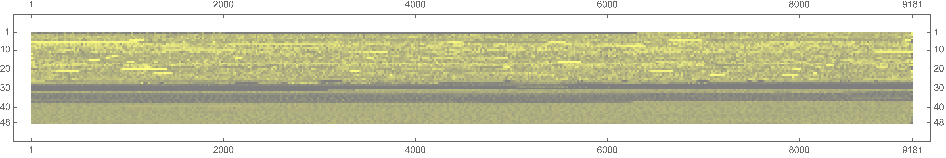
\includegraphics[width=\textwidth]{gr3d}
    \caption{Visualización de los bytes del archivo
original. $M$}
    \label{fig:DatosOrigM1}
\end{figure}

\begin{figure}[H]
    \centering
    
\includegraphics[width=\textwidth]{bytes2}
    \caption{Visualización de los bytes del archivo
cifrado. $N$}
    \label{fig:DatosOrigM2}
\end{figure}\oplus\odot

Todos los puntos grises y amarillos de la figura \ref{fig:DatosOrigM3} son los
bytes que no cambiaron, si lo hicieron los suficientes para que el archivo no
sea reconocible por ningún programa como el ejecutable que era.

\begin{figure}[H]
    \centering
    
\includegraphics[width=\textwidth]{bytes3}
    \caption{$M-N$}
    \label{fig:DatosOrigM3}
\end{figure}

Para quien abre el archivo, las claves de qué se trata son pocas, aún más
desconociendo la existencia de la herramienta (\texttt{lcy})

Para descifrar el archivo solo se necesita usar el comando:

\begin{minted}{rust}
    lcy decipher texto.txt.lcy
\end{minted}

Lo que crea un archivo llamado \texttt{texto.txt} que contiene:

\begin{minted}{rust}
Este es un mensaje super secreto!

\end{minted}

\newpage
\section{Discusión de Resultados}

\subsection{Descifrado por histogramas}

La mayor vulnerabilidad que presenta este método de cifrado es que la
frecuencia de bytes presentes es la misma debido a que no estamos
sacrificando ninguna pérdida de información y, por lo tanto, solo sustituimos
los
valores.

\begin{figure}[H]
    \centering
    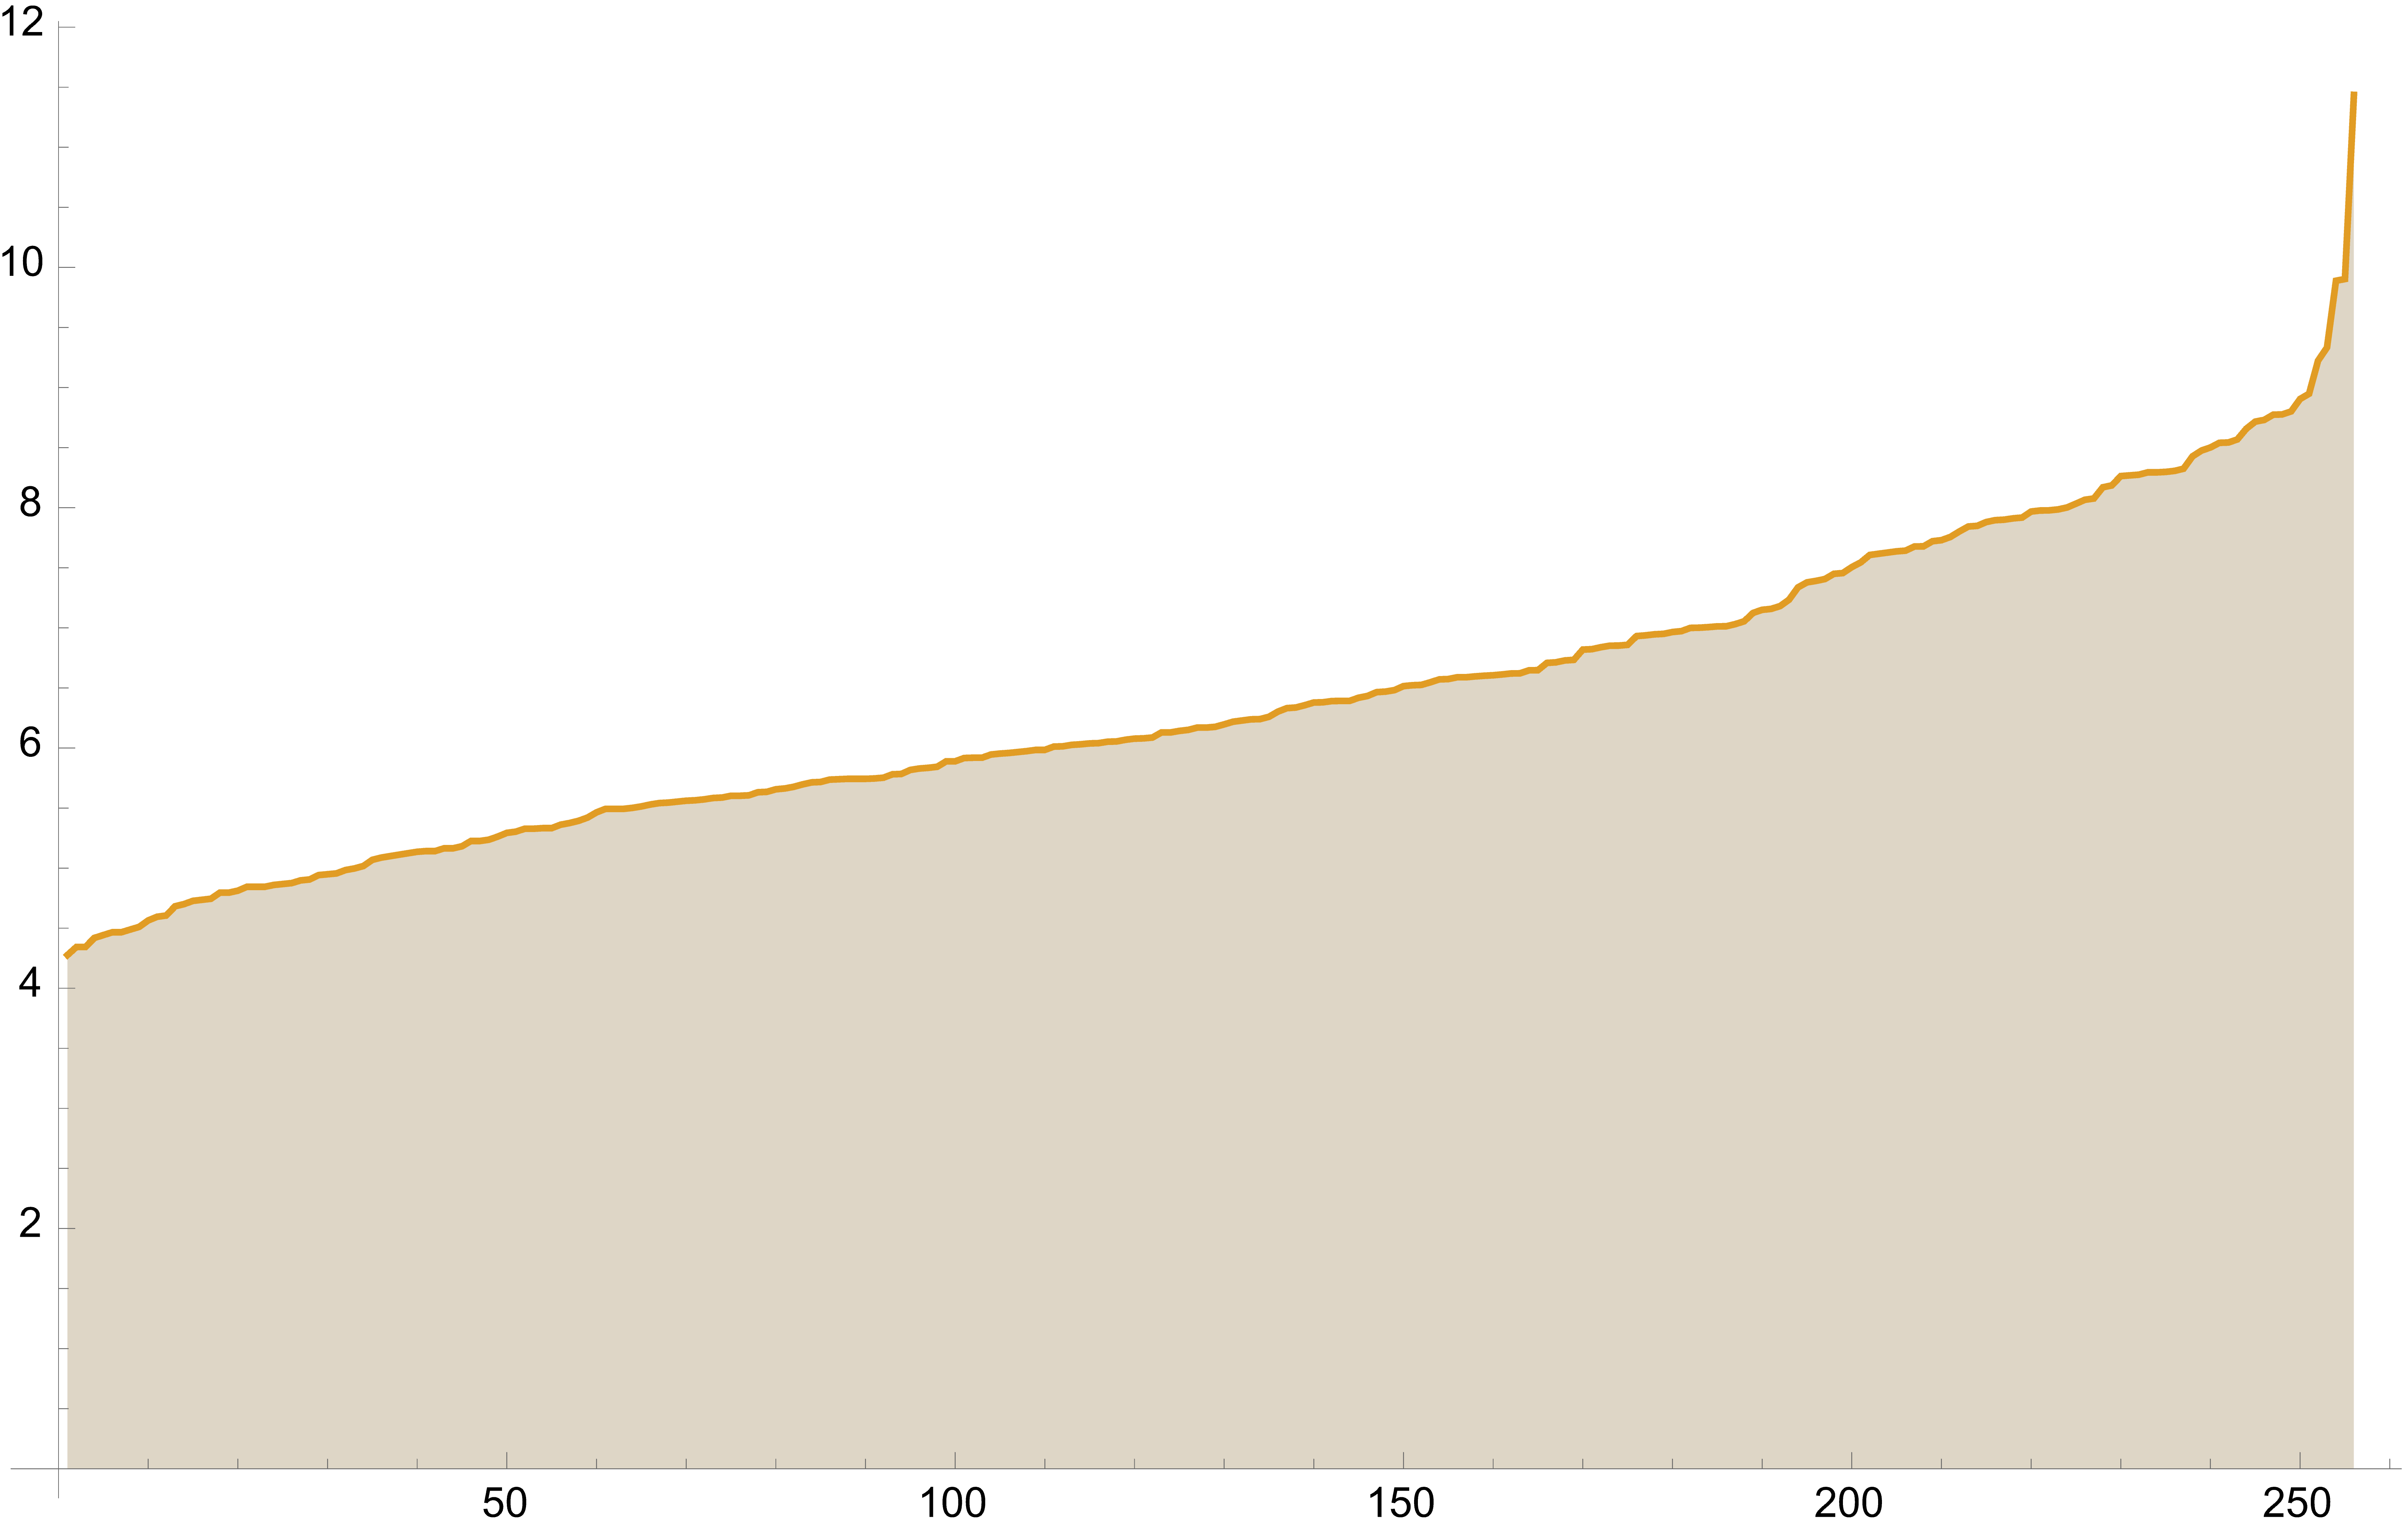
\includegraphics[width=\textwidth]{historygram.png}
    \caption{Histograma de los bytes del archivo
original y el cifrado.}
    \label{fig:Histo1}
\end{figure}

En la figura \ref{fig:Histo1}, se muestra la sobre posición de los histogramas
de bytes del documento antes y después de cifrado. Ambos son idénticos. Si el
documento está escrito en Inglés o contuviera las instrucciones de cierta
arquitectura, y se conoce la frecuencia de bytes, el mensaje puede ser
descifrado.

Todo lo anterior en caso de que el posible atacante supiera que el cifrado se
hace desde nivel de bytes. Si alguien intentara hacer un histograma de los
caracteres del archivo original con el cifrado se encontraría con:

\begin{figure}[H]
    \centering
    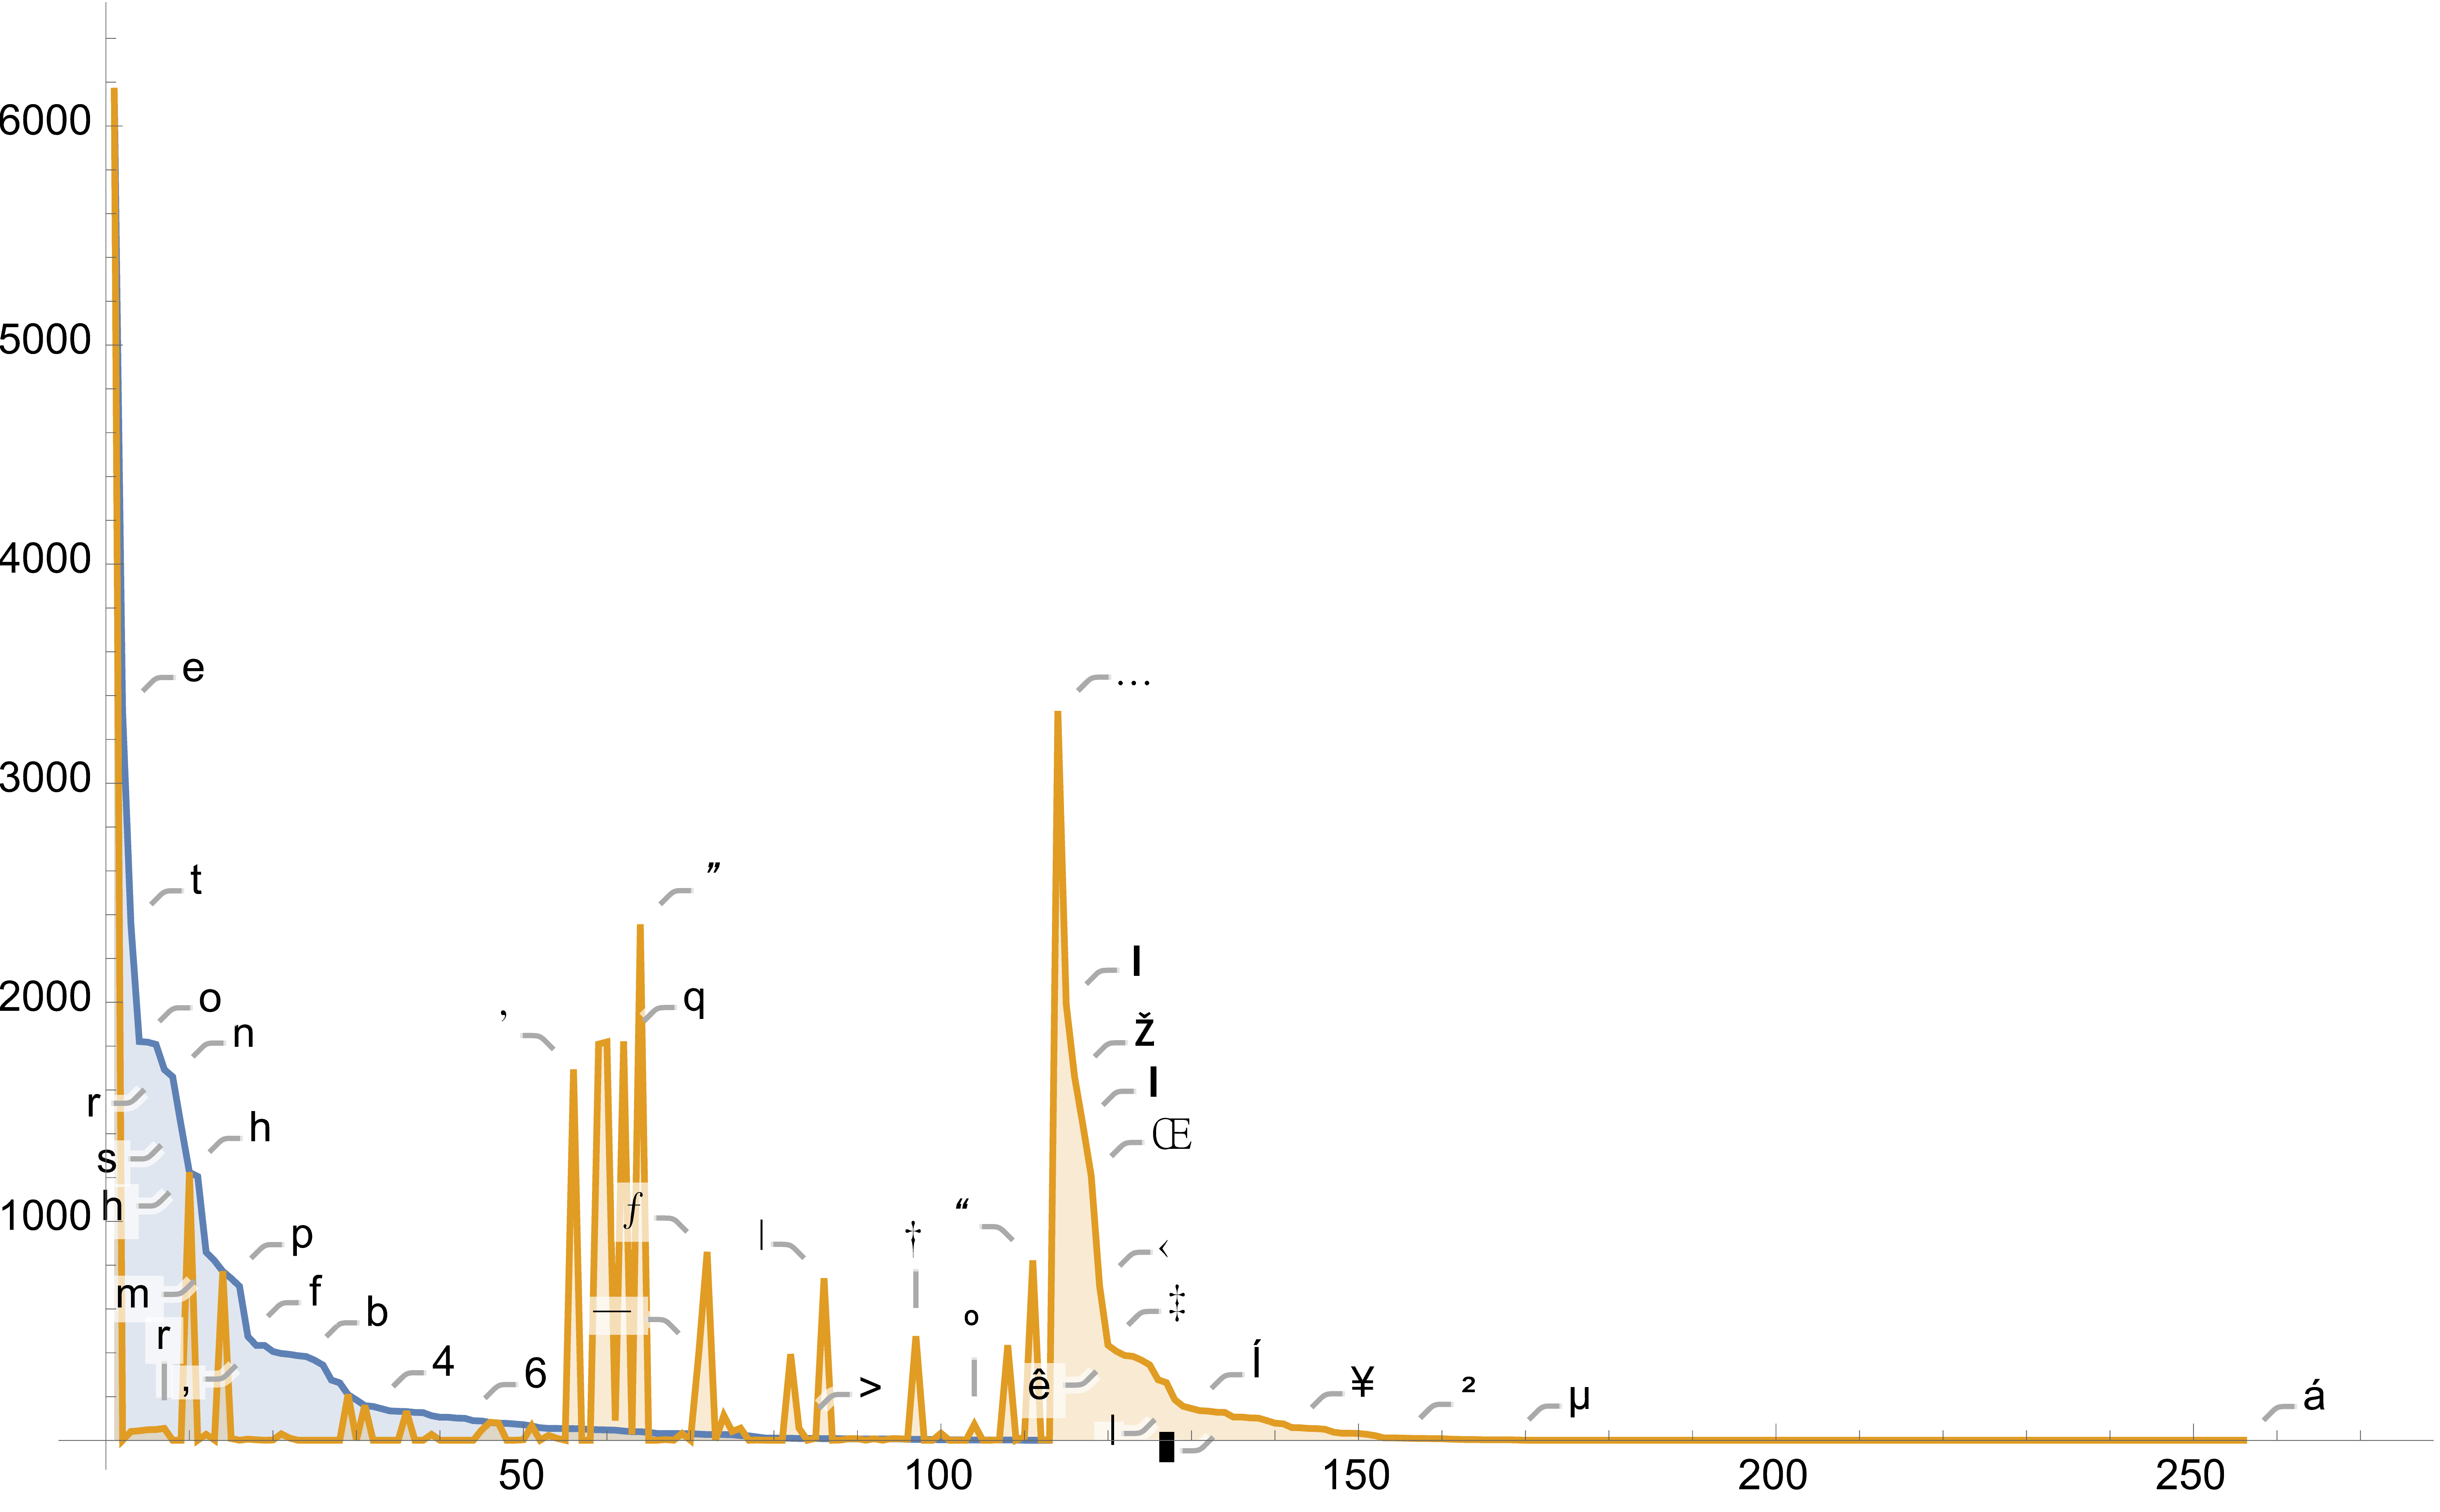
\includegraphics[width=\textwidth]{histo2}
    \caption{Histograma de los caracteres humanamente leíbles del archivo
original y el cifrado.}
    \label{fig:Histo2}
\end{figure}

Si ordenamos por aparición y aplicamos el logaritmo natural de los valores es
más fácil apreciar:

\begin{minted}{wolfram}
With[
 {assoc = CharacterCounts[baa], assoc2 = CharacterCounts[bxx]},
  ListLinePlot[
  {
   Log[KeySortBy[assoc, assoc[#] &]],
   Log[KeySortBy[assoc2, assoc2[#] &]]
   },
  
  Filling -> Axis, PlotRange -> Full, ImageSize -> Large
  ]
 ]
\end{minted}

\begin{figure}[H]
    \centering
    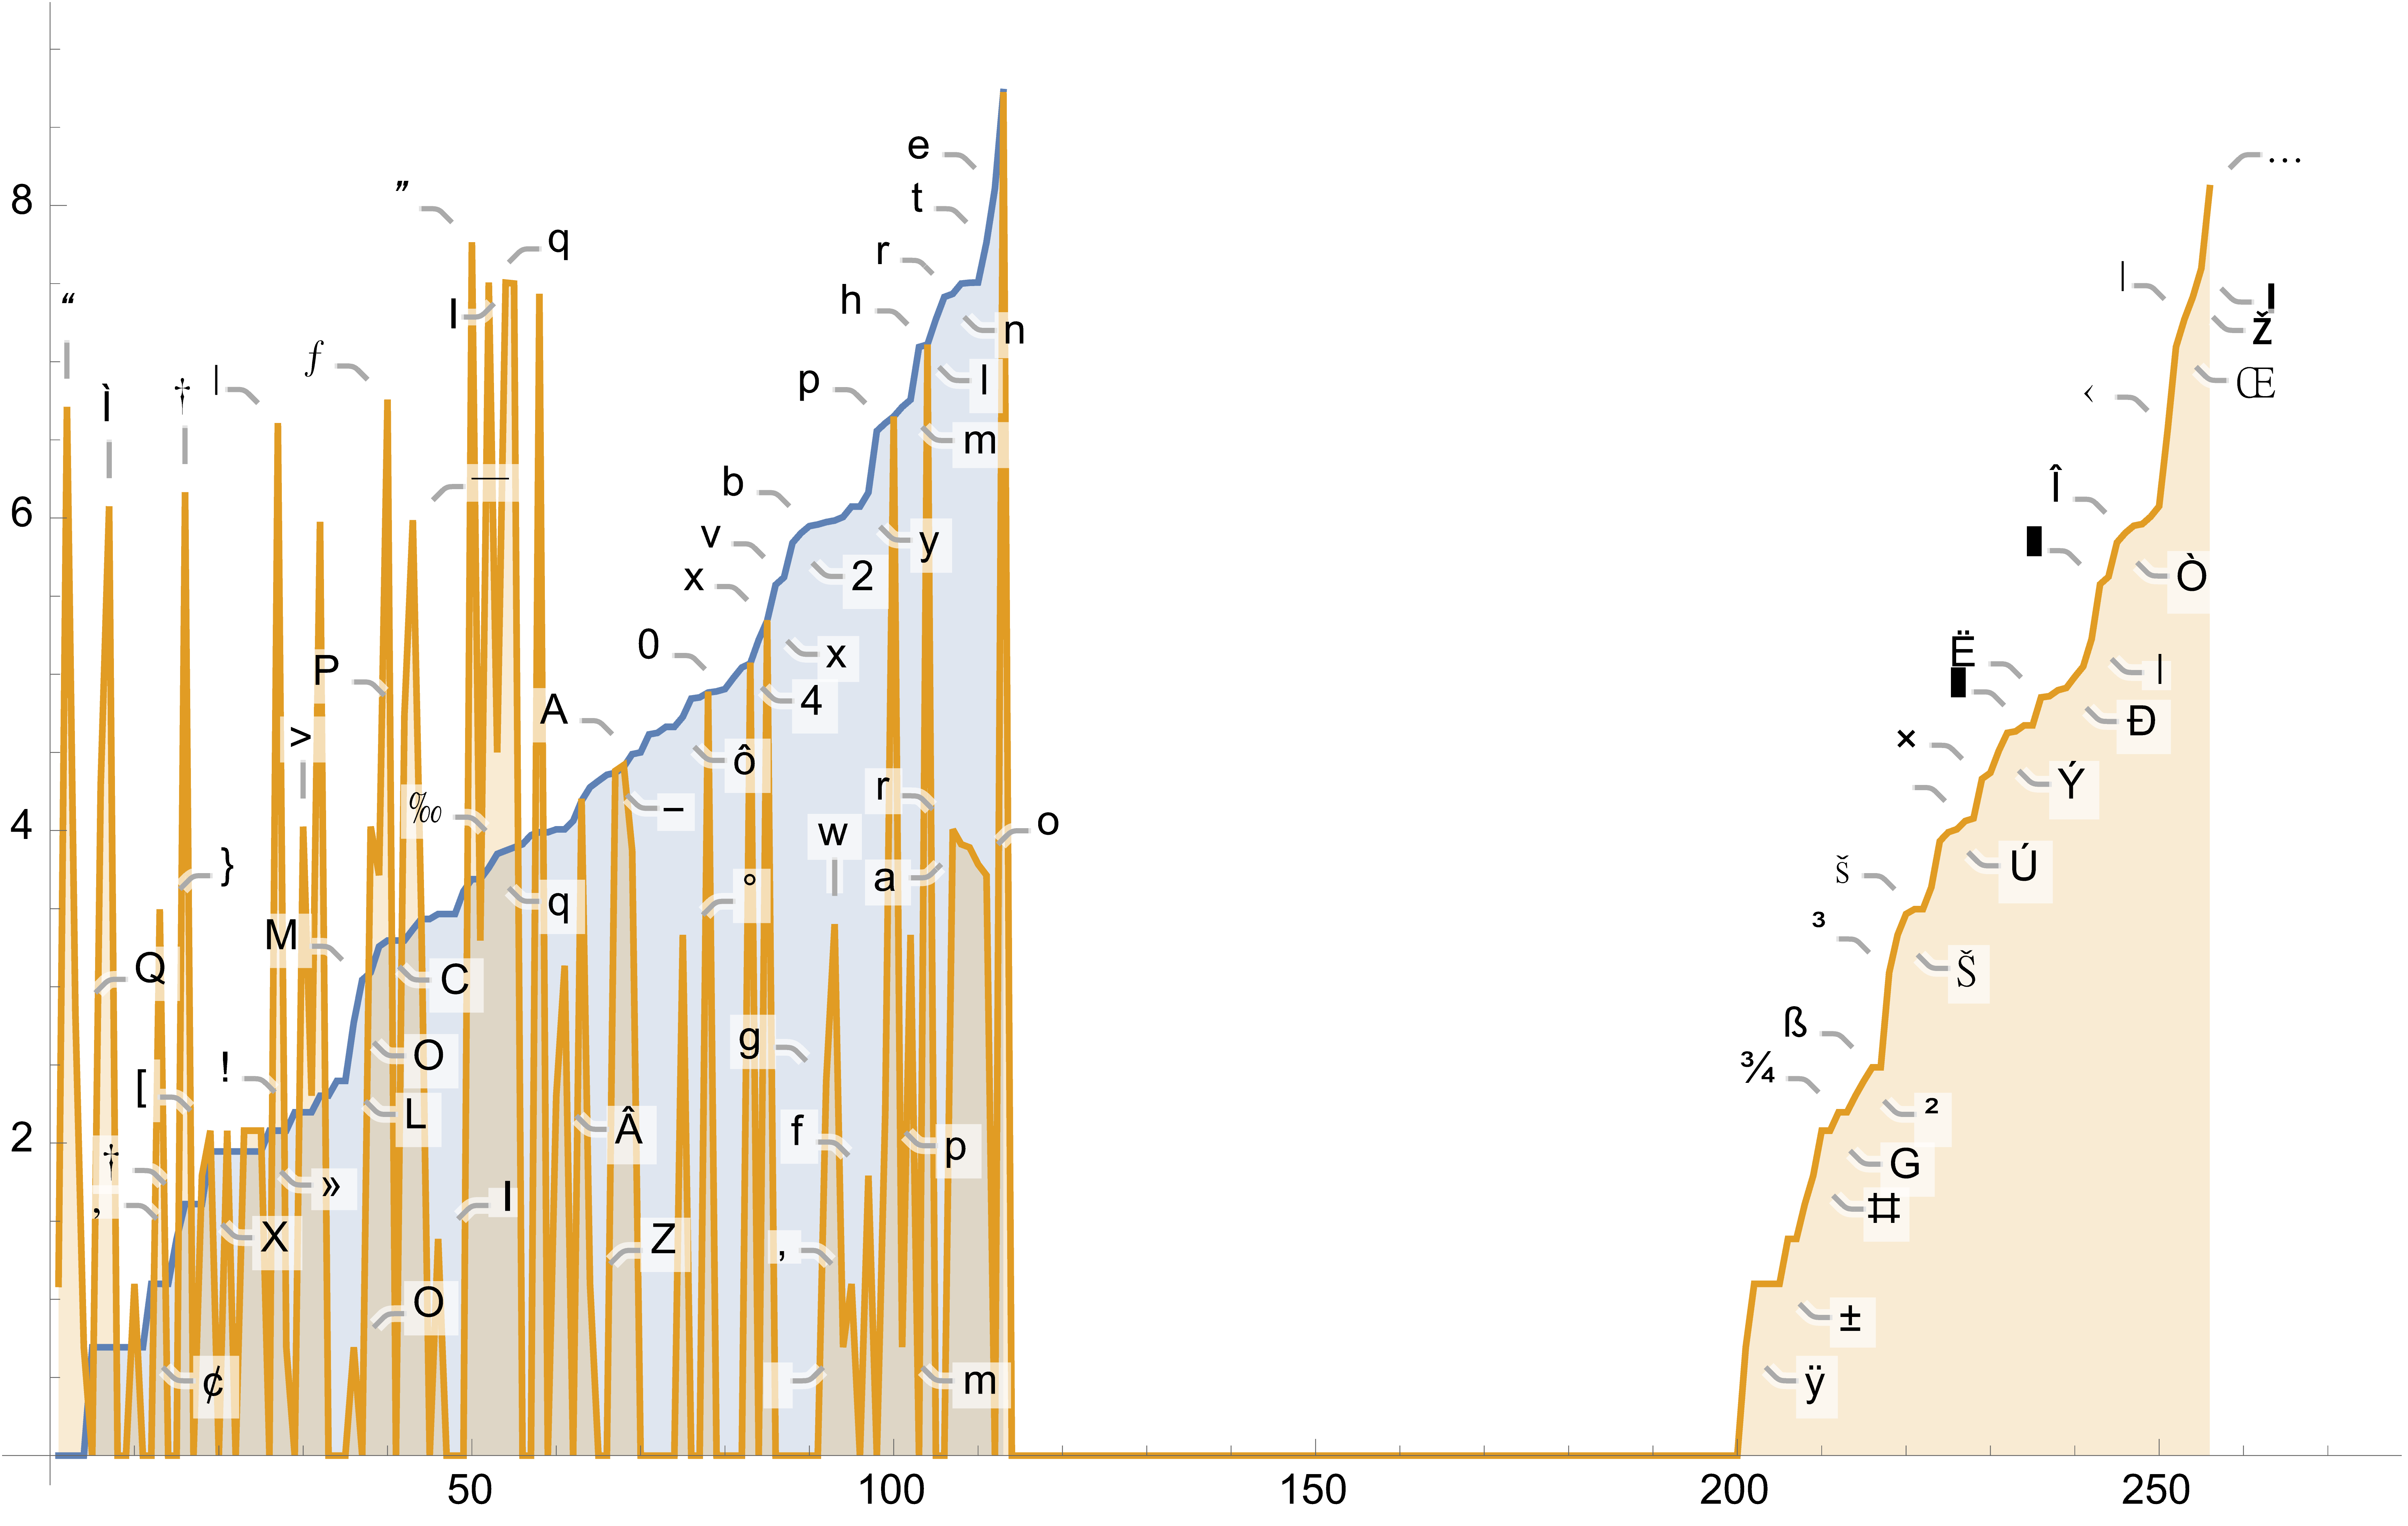
\includegraphics[width=\textwidth]{histo1}
    \caption{Histograma de los caracteres humanamente leíbles del archivo
original y el cifrado.}
    \label{fig:Histo0}
\end{figure}


Donde es claro el caos resultado del cifrado del archivo. En la situación donde
alguien malicioso desee descifrarlo por comparación de histogramas de
caracteres, no hay posibilidad de que sea logrado.

El método 2, aunque promete ser aún más seguro permitiendo la generación de
histogramas sin ningún sentido, requiere más recursos del computador donde se
utiliza. Si se quiere cifrar una base de datos de 1 GB se necesitará
aproximadamente 200 MB para contener los archivos además de la memoria
necesaria para manejar la creación de la matriz aleatoria en el tiempo de
ejecución.

El método 1 es más \textit{ligero} en comparación al método 2 aunque signifique
que es más seguro de romper.

\subsection{Vulnerabilidades de almacenamiento}

La herramienta que desarrollamos almacena y captura los datos de cifrado del
mismo archivo donde se encuentra el cifrado, por ello, cualquier persona que
sepa que se usó \texttt{lcy} para cifrar el archivo puede descifrar el archivo.
Hace falta algún sistema de contraseñas, puede que a cada tecla se le pueda
asignar una transformación sencilla que se genera aleatoriamente. 

De forma en que el algoritmo cifrado pasaría a ser:

\[
\text{BytesCifrados} \times T^{-1} \times Pass \equiv \text{Bytes}
\]

Otra forma de ampliar la seguridad de la herramienta es escribir en múltiples
archivos. 

Un archivo para la inversa de la transformación, un archivo para
\text{BytesCifrados} y un archivo para el mensaje cifrado en lugar de colocarlo
en uno solo, de esa forma sólo el usuario que cifra el mensaje sabe cuáles son
los archivos necesarios para descifrarlo en su computador.

\newpage
\section{Conclusiones y Recomendaciones}

Como pudimos observar en todo el documento la importancia del algebra lineal en
nuestras vidas cotidianas, como pueden ser en distintos aspectos, aunque en
esta ocasión nos quisimos centrar en la importancia que tiene este en la
ciberseguridad.

Pero viviendo en una época en donde ocurren muchos ataques y como cualquier
persona almacena cualquier tipo de información en sus dispositivos móviles o en
sus computadoras, una capa más de seguridad no afectaría a nadie.

Las transformaciones resultan una herramienta invaluable para producir
algoritmos sencillos y efectivos de cifrado y descifrado de archivos, imágenes,
etc. Es trivial manipular la información cuando se razona desde el punto de
vista de ser una matriz.

Está claro que falta explorar más formas de desarrollar el algoritmo para
disminuir las posibilidades de que agentes externos entiendan información
sensible que se encuentre almacenada.

Entre las mejoras a implementar se encuentra eliminar la posibilidad de
descifrado por medio de histogramas de los bytes. Creemos que el método 2
estudiado en la experimentación es capaz de lograrlo.

Además, mejorar la base de código para que cada pieza necesaria sea almacenada
en un archivo distinto para ser usados como llaves y la posibilidad de asociar
matrices a caracteres para aumentar la seguridad aún más.

Aunque se cumplió el objetivo de implementar una herramienta de cifrado y
descifrado
a
nivel de bytes usando transformaciones y matrices, creemos que queda abierto el
espacio para seguir investigando.

\newpage
\section{Bibliografía}
\printbibliography[heading=none]

\newpage

\appendix

\section{Appendix}

Comparación de histograma de las ocurrencias de bytes entre un arreglo de bytes
y su versión cifrada por el \texttt{Método 1}

\begin{figure}[H]
    \centering
    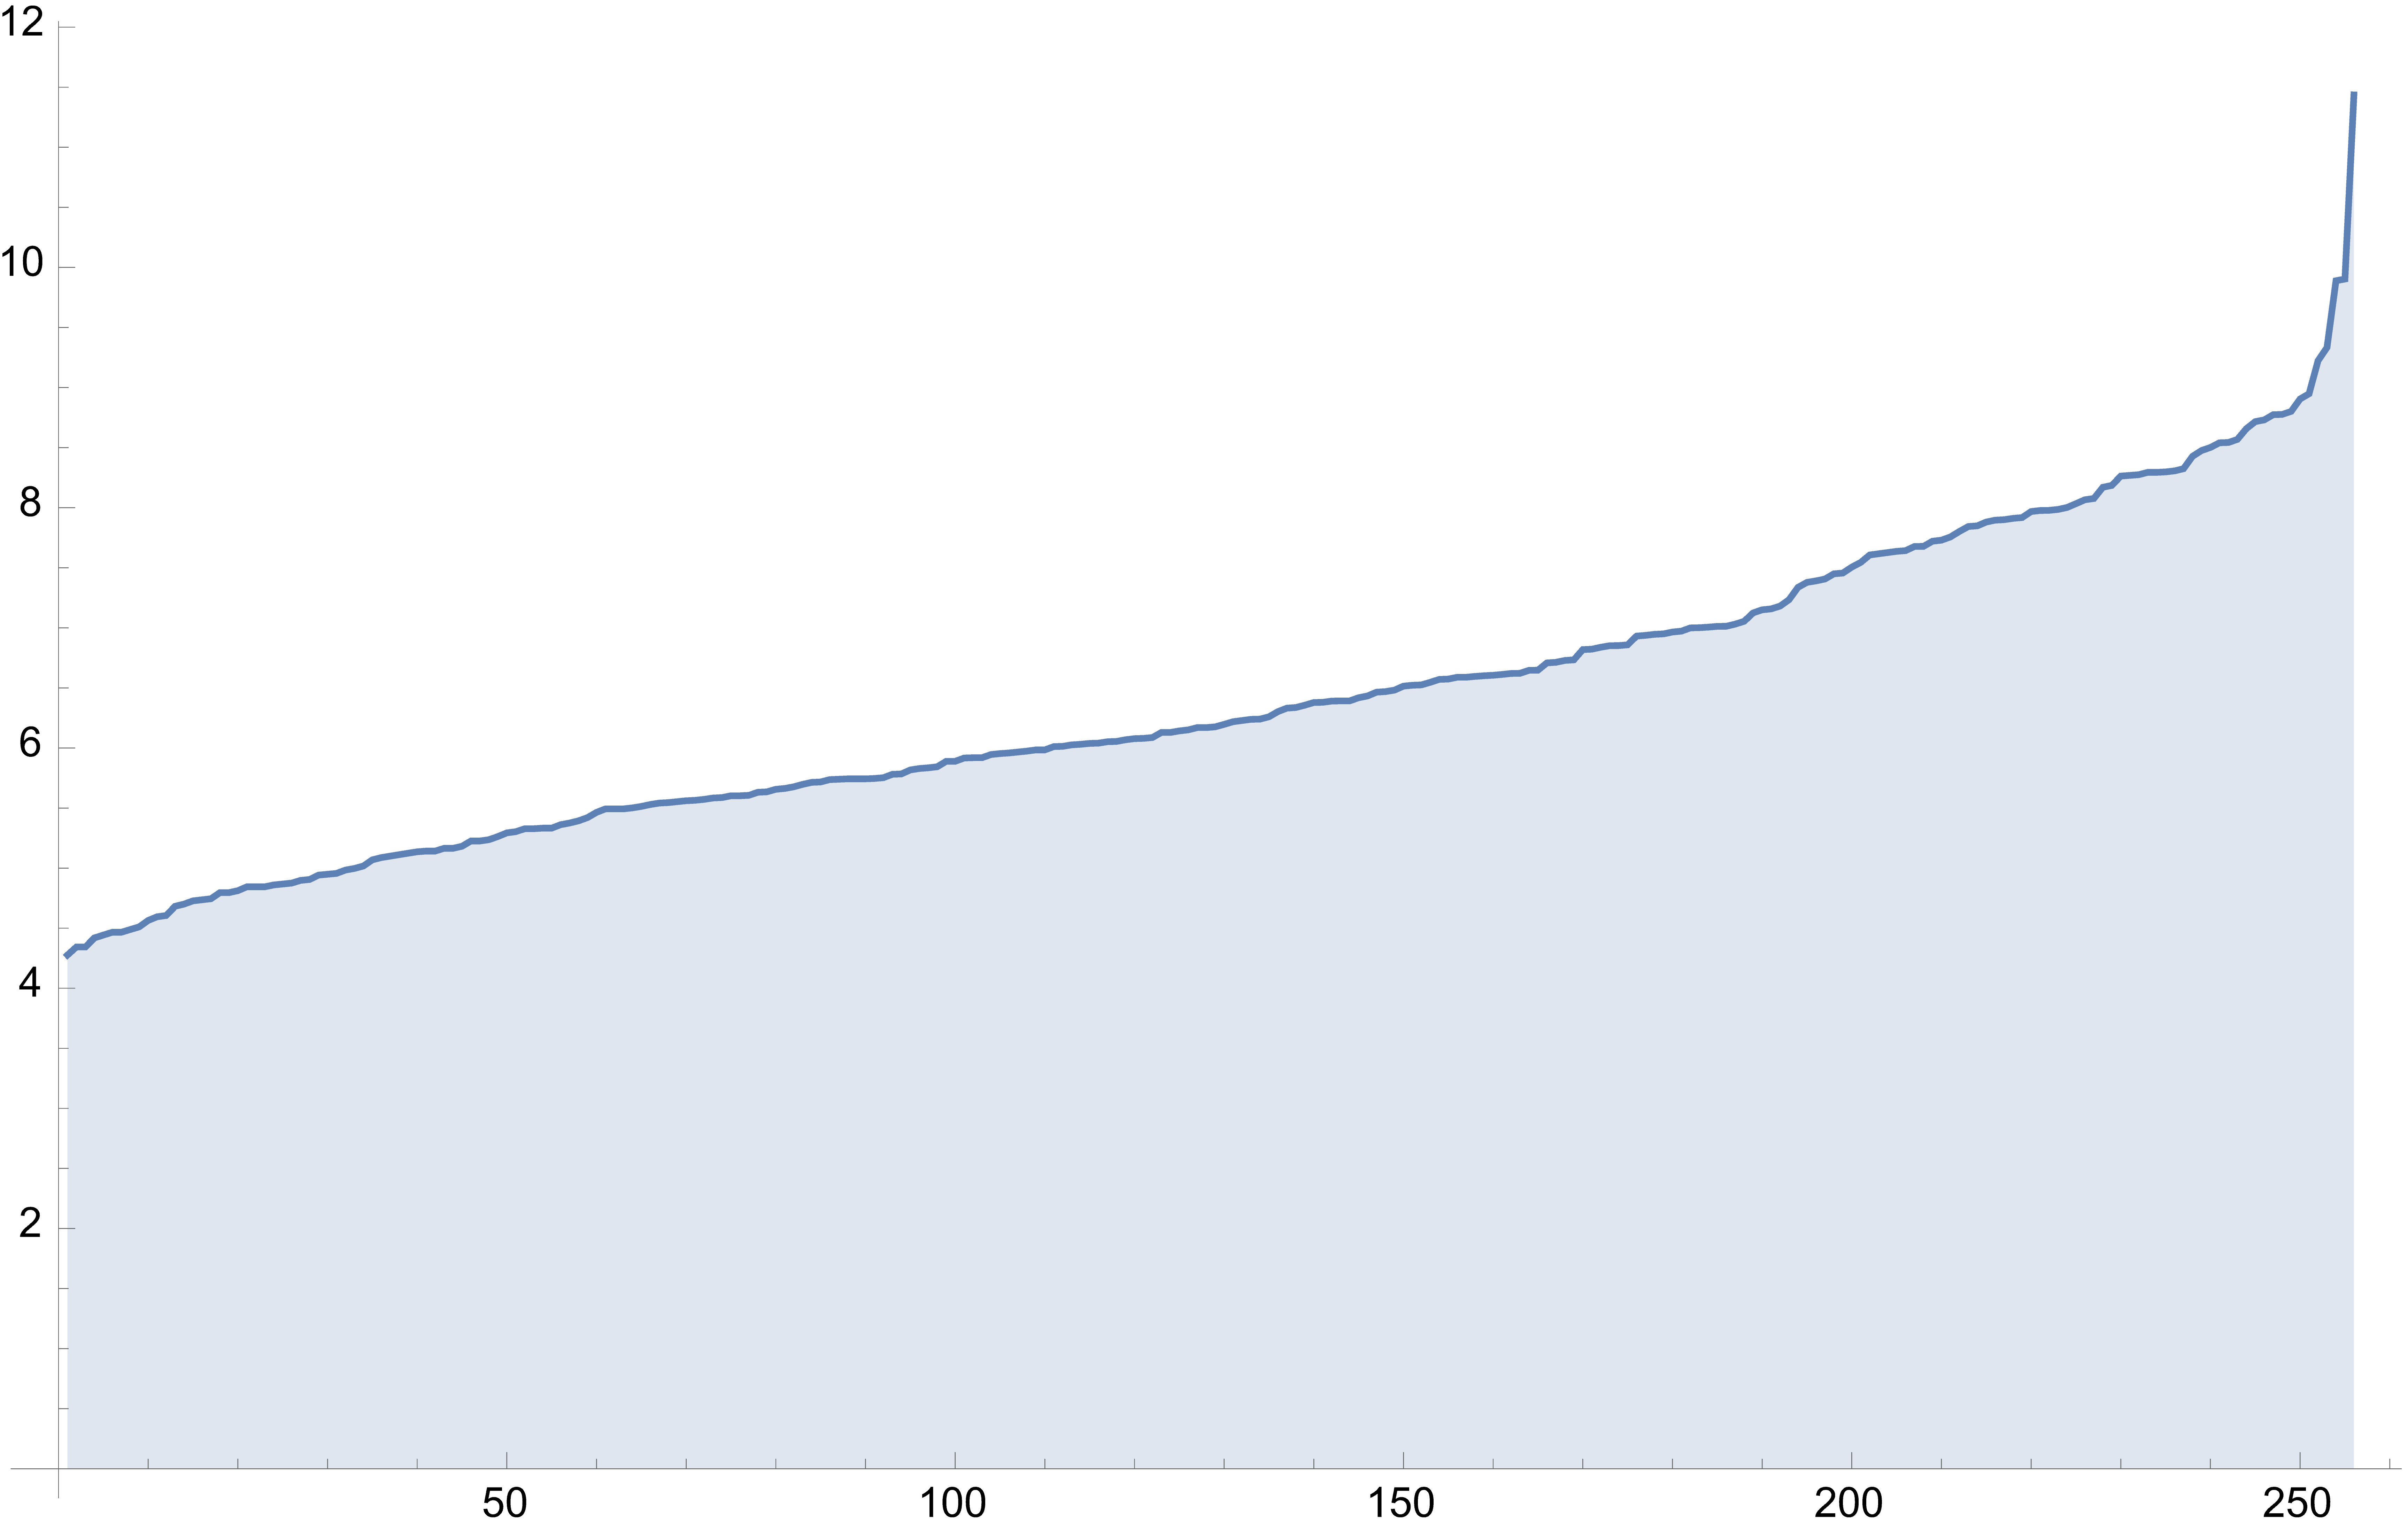
\includegraphics[scale=0.7]{historygramorig}
    \caption*{Histograma de los bytes del archivo
original y el cifrado.}\label{fig:d1}
\end{figure}

\begin{figure}[H]
    \centering
    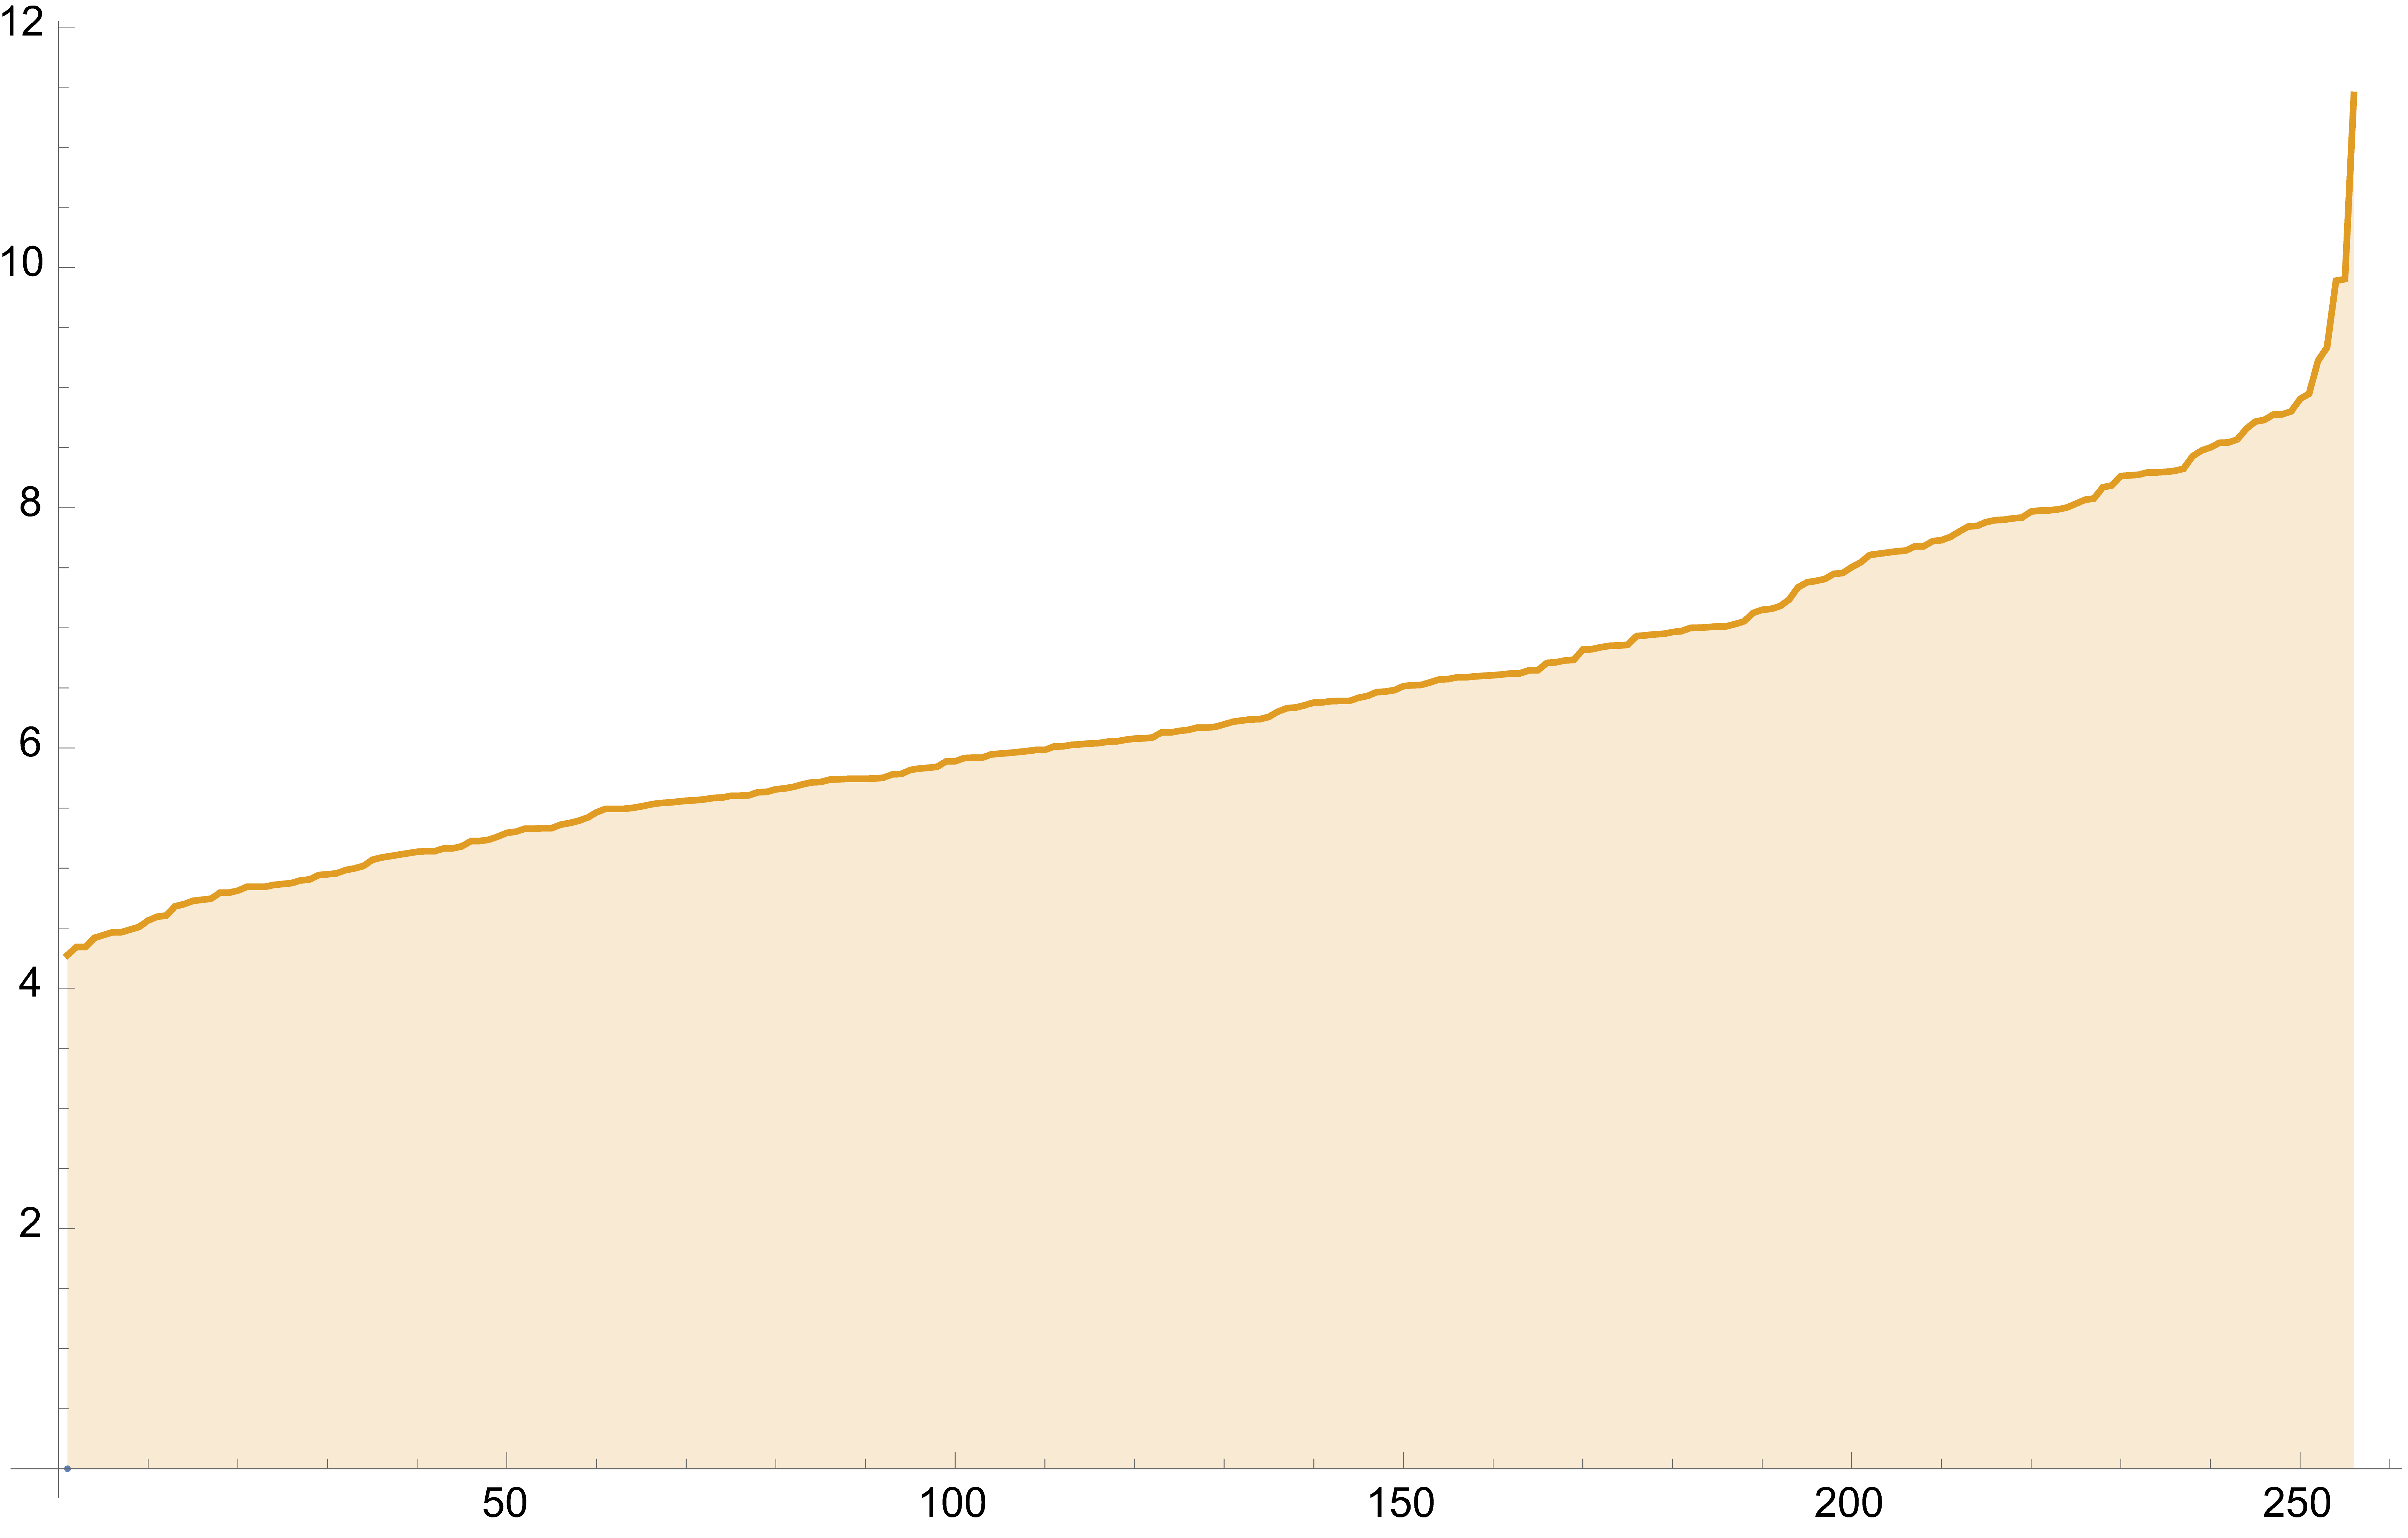
\includegraphics[scale=0.7]{historygramorig2}
    \caption*{Histograma de los bytes del archivo cifrado.}
    \label{fig:d3}
\end{figure}

\begin{figure}[H]
    \centering
    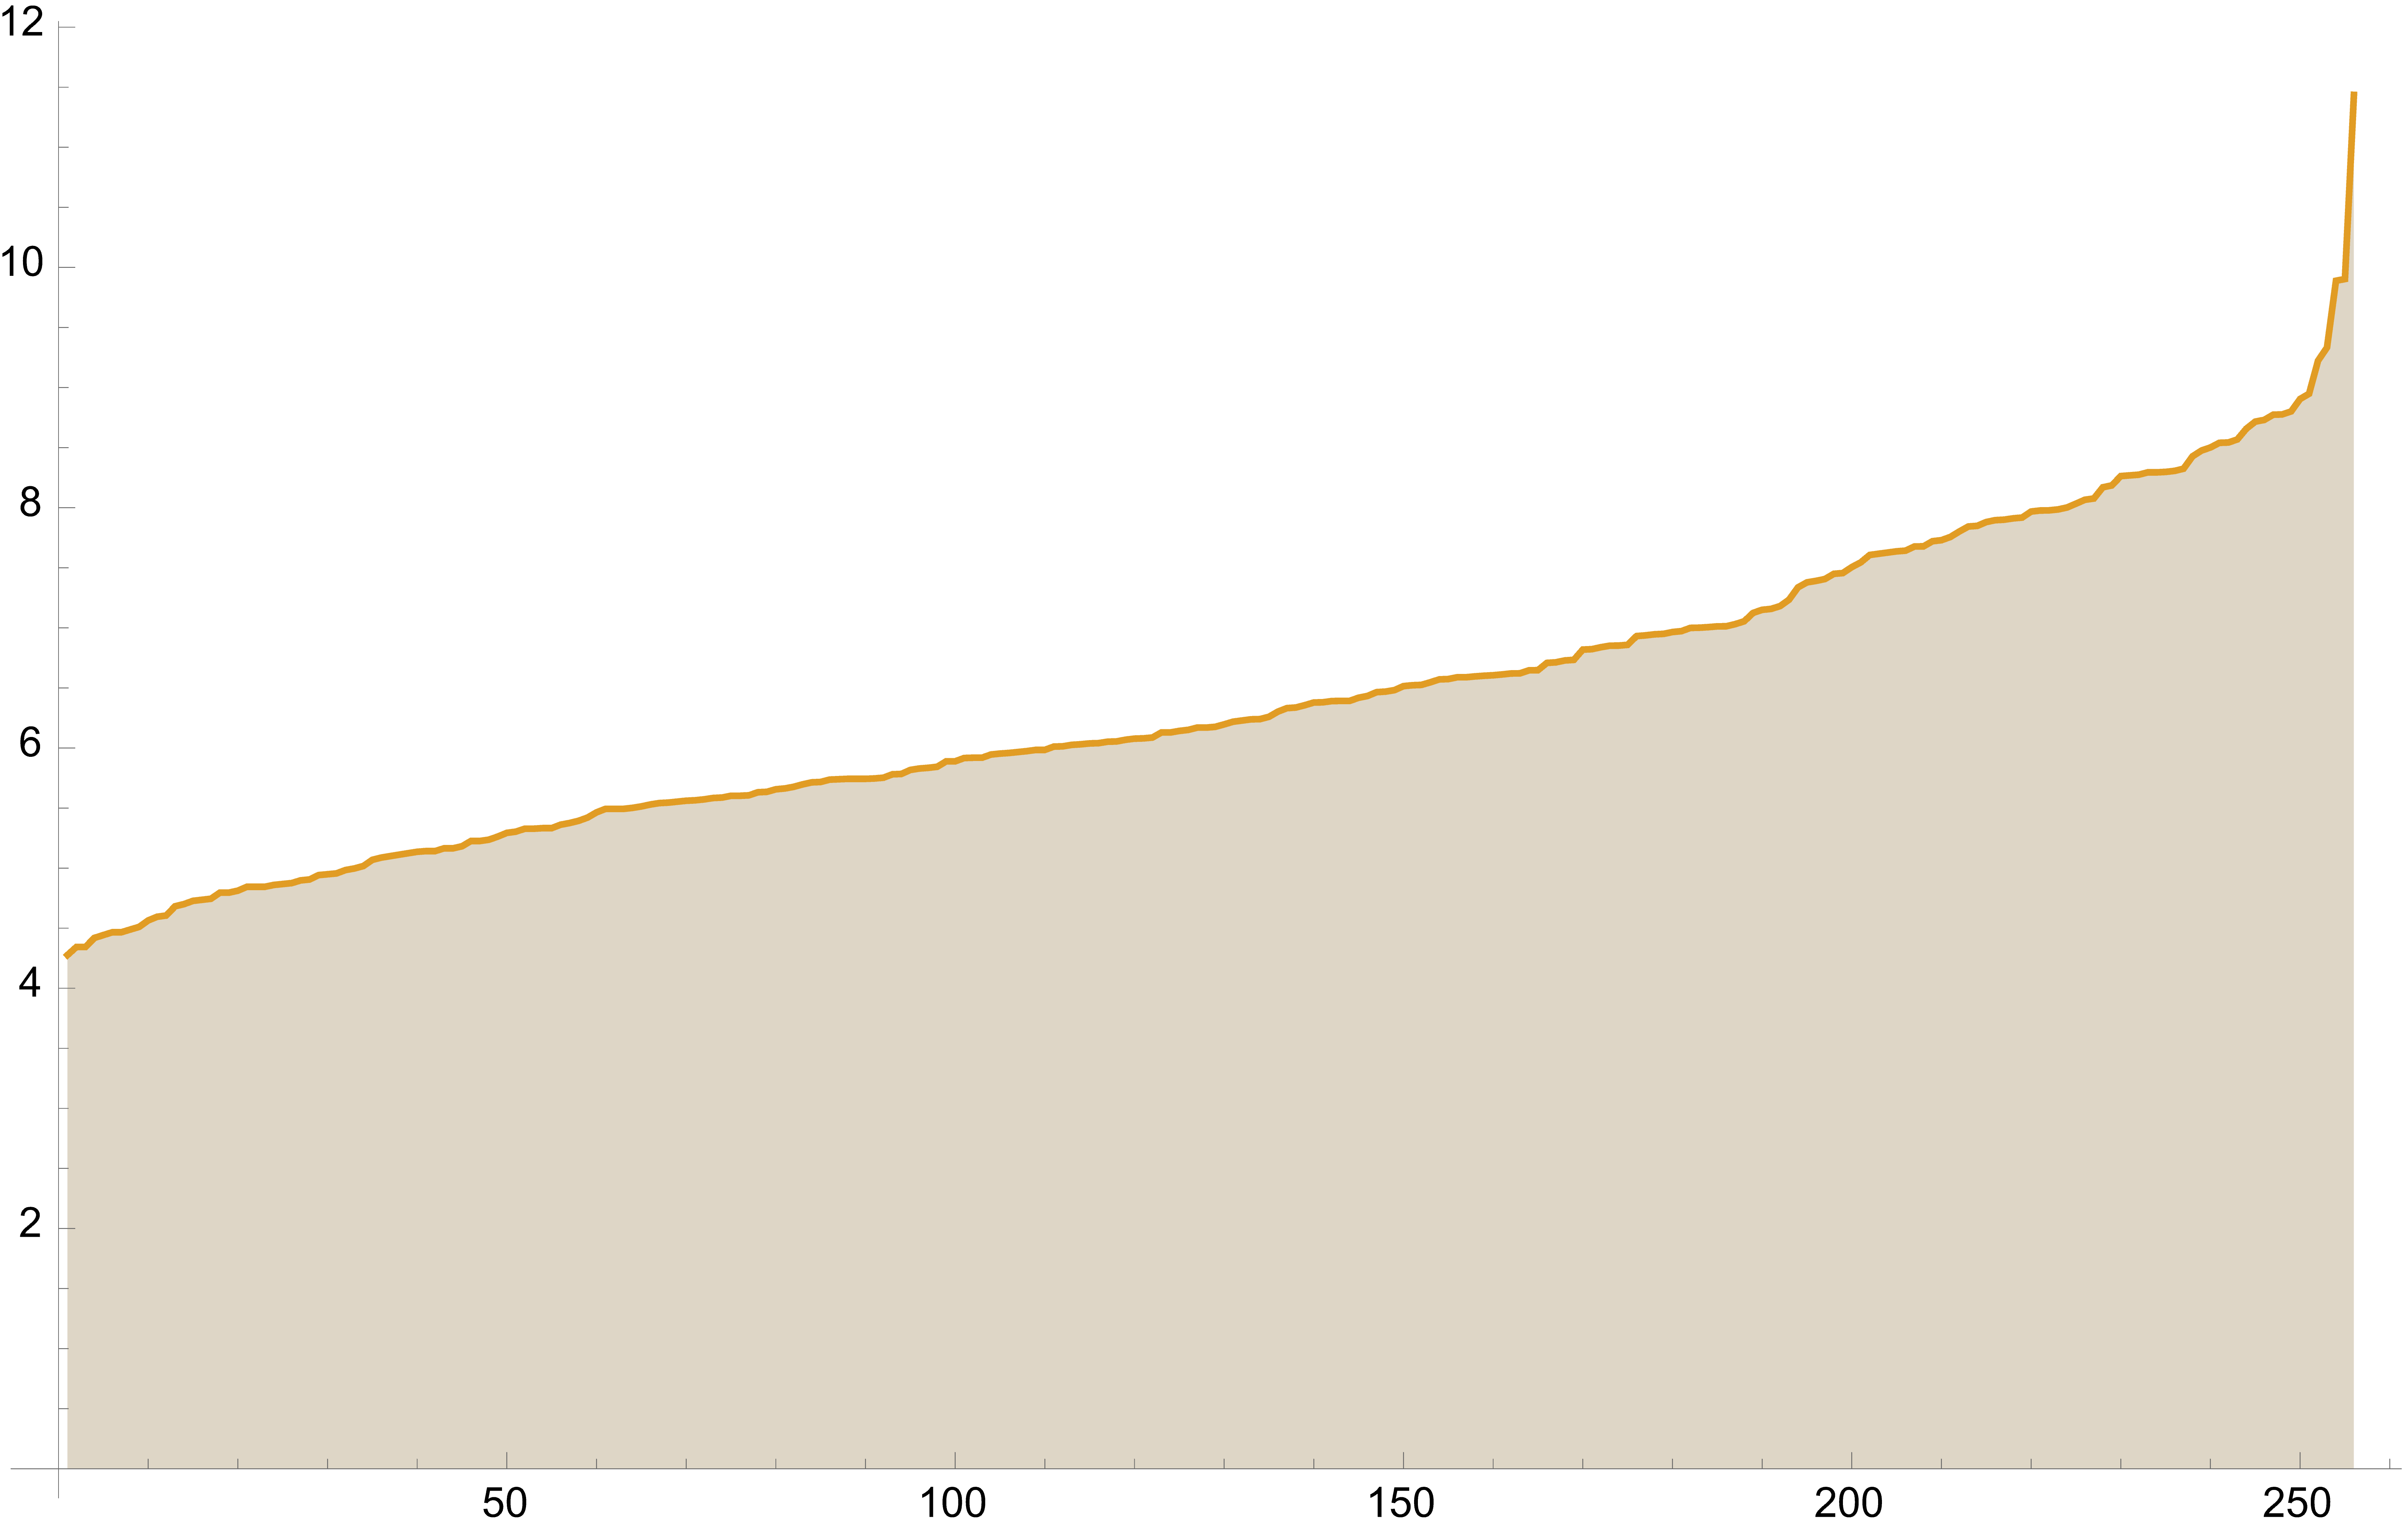
\includegraphics[scale=0.7]{historygram}
    \caption*{Histograma de los bytes del archivo
original y el cifrado.}\label{fig:d2}
\end{figure}

Gráficas elaboradas en Mathematica 13 con el código:

\begin{minted}[linenos]{wolfram}
Show[
    With[
        {
            assoc = CountRepetitions[baa],
            assoc2 = CountRepetitions[Flatten[bx]]
        },

        ListLinePlot[
            {
                KeyValueMap[Log[#2] &]@KeySortBy[assoc, assoc[#] &],
                KeyValueMap[Log[#2] &]@KeySortBy[assoc2, assoc2[#] &]
            },
            Filling -> Axis,
            PlotRange -> Full,
            ImageSize -> Large
        ]
    ]
]
\end{minted}

donde \texttt{baa} es un arreglo de bytes conteniendo el estado del archivo
original y donde \texttt{bx} es una matriz que se usa como arreglo de bytes que
contiene el estado cifrado de los contenidos de donde \texttt{baa}.

\newpage
\section{Appendix}

\begin{minted}[linenos]{rust}
pub fn met1_armar_matriz(rng: &mut ThreadRng) -> DMatrix<f32> {
    let mut resultado: DMatrix<f32> = dmatrix![].resize(32, 32, 0.0);

    let mut switch: [bool; 32] = [false; 32];
    let mut neg: [bool; 32] = [false; 32];

    for col in 1..32 / 2 {
        if rng.gen::<u8>() % 2 == 0 {
            switch[col] = true;
            switch[31 - (col - 1)] = true;
        }

        if rng.gen::<u8>() % 5 == 0 {
            neg[col] = true;
            neg[31 - (col - 1)] = true;
        }
    }

    resultado[(0, 0)] = 1.0;

    for col in 1..32 {
        if switch[col] {
resultado[(col, 31 - (col - 1))] = if neg[col] { 1.0 } else { -1.0 };
        } else {
            resultado[(col, col)] = if neg[col] { 1.0 } else { -1.0 };
        }
    }

let switch_mat: DMatrix<bool> = DMatrix::from_vec(1, 32, Vec::from(switch));

    resultado
}
\end{minted}

\newpage
\section{Appendix}

\begin{minted}[linenos]{rust}
extern crate nalgebra as na;

use divisors::get_divisors;
use lcy::*;
use std::collections::HashMap;
use std::fs::{remove_file, OpenOptions};
use std::io::{Read, Seek, Write};
use std::process::exit;

use na::{dmatrix, DMatrix};

fn main() {
    let mut rng = rand::thread_rng();
    let args: Args = Args::parse();

    let mut map: HashMap<u8, u8> = HashMap::new();

    match args.command {
        Commands::Cypher { path } => {
            let bytes: DMatrix<f32> = dmatrix![ ... ];

            if !path.exists() {
                eprintln!("Error: El archivo {} no existe!", path.display());
                exit(1)
            }

            let mut file = OpenOptions::new()
                .read(true)
                .write(true)
                .create(false)
                .open(&path)
                .unwrap();

            let mut file2 = OpenOptions::new()
                .write(true)
                .create(true)
                .truncate(true)
                .open(&format!("{}.lcy", &path.display()))
                .unwrap();

            let mut contenidos: Vec<u8> = vec![];

            file.read_to_end(&mut contenidos).unwrap();

            let mat = met1_armar_matriz(&mut rng);
            let mut key = &bytes * &mat;
            let inv_key = mat.clone().try_inverse().unwrap();

            for i in 0..8usize {
                for j in 0..32usize {
                    key[(i, j)] = key[(i, j)].rem_euclid(256.0);
                    map.insert(bytes[(i, j)] as u8, key[(i, j)] as u8);
                }
            }

            for i_byte in 0..contenidos.len() {
                contenidos[i_byte] = *map.get(&contenidos[i_byte]).unwrap();
            }

            let mut inv_key_to_write = vec![];
            let mut bytes_final_to_write = vec![];
            for i in 0..32 {
                for j in 0..32 {
let indicador = if inv_key[(i, j)] < 0.0 { 1u8 } else { 0u8 };
                    let val = if inv_key[(i, j)] < 0.0 {
                        -1.0 * inv_key[(i, j)]
                    } else {
                        inv_key[(i, j)]
                    };

                    inv_key_to_write.push(indicador);
                    inv_key_to_write.push(val as u8);
                }
            }

            for i in 0..8 {
                for j in 0..32 {
                    bytes_final_to_write.push(key[(i, j)] as u8);
                }
            }

            file2.write_all(&[66u8, 60u8, 10u8, 255u8]).unwrap();
            file2.write_all(&inv_key_to_write).unwrap();
            file2.write_all(&bytes_final_to_write).unwrap();
            file2.write_all(&contenidos).unwrap();

            remove_file(path).unwrap();
        }
        Commands::Decipher { path } => { ... }
    }
}
\end{minted}

\newpage
\section{Appendix}

\begin{minted}[linenos]{rust}
extern crate nalgebra as na;

use divisors::get_divisors;
use lcy::*;
use std::collections::HashMap;
use std::fs::{remove_file, OpenOptions};
use std::io::{Read, Seek, Write};
use std::process::exit;

use na::{dmatrix, DMatrix};

fn main() {
    let mut rng = rand::thread_rng();
    let args: Args = Args::parse();

    let mut map: HashMap<u8, u8> = HashMap::new();

    match args.command {
        Commands::Cypher { path } => { ... }
        Commands::Decipher { path } => {
            if !path.exists() {
                eprintln!("Error: El archivo {} no existe!", path.display());
                exit(1)
            }

let orig_path = path.as_os_str().to_str().unwrap().replace(".lcy", "");

            let mut file_ci = OpenOptions::new()
                .read(true)
                .write(true)
                .create(false)
                .open(&path)
                .unwrap();

            let mut file = OpenOptions::new()
                .read(true)
                .write(true)
                .truncate(true)
                .create(true)
                .open(&orig_path)
                .unwrap();

            let mut contenidos: Vec<u8> = vec![];

            file_ci.read_to_end(&mut contenidos).unwrap();

            if contenidos[0..0x4] != [66u8, 60u8, 10u8, 255u8] {
                eprintln!("Error: No es un archivo válido cifrado");
                exit(1);
            }

            let mut inv = dmatrix![].resize(32, 32, 0.0);
            let mut key = dmatrix![].resize(8, 32, 0.0);

            let contenidos = &contenidos[0x4..];

            let mut k = 0;
            for i in 0..32 {
                for j in 0..32 {
                    let neg = contenidos[k] == 0x1;
let val = (contenidos[k + 1] as i32) * if neg { -1 } else { 1 };

                    inv[(i, j)] = val as f32;
                    k += 2;
                }
            }

            let contenidos = &contenidos[k..];

            let mut k = 0;
            for i in 0..8 {
                for j in 0..32 {
                    key[(i, j)] = contenidos[k] as f32;
                    k += 1;
                }
            }

            let mut orig = &key * &inv;

            for i in 0..8usize {
                for j in 0..32usize {
                    orig[(i, j)] = orig[(i, j)].rem_euclid(256.0);
                    map.insert(key[(i, j)] as u8, orig[(i, j)] as u8);
                }
            }

            let mut contenidos = contenidos[k..].to_vec();

            for i_byte in 0..contenidos.len() {
                contenidos[i_byte] = *map.get(&contenidos[i_byte]).unwrap();
            }

            file.write_all(&contenidos).unwrap();
            remove_file(path).unwrap();
        }
    }
}
\end{minted}

\newpage
\section{Appendix: Código completo}

El código está también disponible en GitHub:
\texttt{https://github.com/AOx0/lcy}

\begin{minted}[linenos]{rust}
extern crate nalgebra as na;

use std::collections::HashMap;
use std::fs::{remove_file, OpenOptions};
use std::io::{Read, Write};
use std::process::exit;

use na::{dmatrix, DMatrix};

pub use clap::{Parser, Subcommand};
use rand::rngs::ThreadRng;
use rand::Rng;
use std::path::PathBuf;

#[derive(Parser)]
#[clap(version)]
pub struct Args {
    #[clap(subcommand)]
    pub command: Commands,
}

#[derive(Subcommand, Debug)]
pub enum Commands {
    /// Cypher any file with lcy
    #[clap(visible_alias = "c")]
    Cypher {
        /// Name of the file to cypher
        path: PathBuf,
    },
    /// Decipher a lcy file
    #[clap(visible_alias = "d")]
    Decipher {
        /// Name of the file to decipher
        path: PathBuf,
    },
}

pub fn met1_armar_matriz(rng: &mut ThreadRng) -> DMatrix<f32> {
    let mut resultado: DMatrix<f32> = dmatrix![].resize(32, 32, 0.0);

    let mut switch: [bool; 32] = [false; 32];
    let mut neg: [bool; 32] = [false; 32];

    for col in 1..32 / 2 {
        if rng.gen::<u8>() % 2 == 0 {
            switch[col] = true;
            switch[31 - (col - 1)] = true;
        }

        if rng.gen::<u8>() % 5 == 0 {
            neg[col] = true;
            neg[31 - (col - 1)] = true;
        }
    }

    resultado[(0, 0)] = 1.0;

    for col in 1..32 {
        if switch[col] {
resultado[(col, 31 - (col - 1))] = if neg[col] { 1.0 } else { -1.0 };
        } else {
            resultado[(col, col)] = if neg[col] { 1.0 } else { -1.0 };
        }
    }

    resultado
}

fn main() {
    let mut rng = rand::thread_rng();
    let args: Args = Args::parse();

    let mut map: HashMap<u8, u8> = HashMap::new();

    match args.command {
        Commands::Cypher { path } => {
            let bytes: DMatrix<f32> = dmatrix![ ... ];

            if !path.exists() {
                eprintln!("Error: El archivo {} no existe!", path.display());
                exit(1)
            }

            let mut file = OpenOptions::new()
                .read(true)
                .write(true)
                .create(false)
                .open(&path)
                .unwrap();

            let mut file2 = OpenOptions::new()
                .write(true)
                .create(true)
                .truncate(true)
                .open(&format!("{}.lcy", &path.display()))
                .unwrap();

            let mut contenidos: Vec<u8> = vec![];

            file.read_to_end(&mut contenidos).unwrap();

            let mat = met1_armar_matriz(&mut rng);
            let mut key = &bytes * &mat;
            let inv_key = mat.clone().try_inverse().unwrap();

            for i in 0..8usize {
                for j in 0..32usize {
                    key[(i, j)] = key[(i, j)].rem_euclid(256.0);
                    map.insert(bytes[(i, j)] as u8, key[(i, j)] as u8);
                }
            }

            for i_byte in 0..contenidos.len() {
                contenidos[i_byte] = *map.get(&contenidos[i_byte]).unwrap();
            }

            let mut inv_key_to_write = vec![];
            let mut bytes_final_to_write = vec![];
            for i in 0..32 {
                for j in 0..32 {
let indicador = if inv_key[(i, j)] < 0.0 { 1u8 } else { 0u8 };
                    let val = if inv_key[(i, j)] < 0.0 {
                        -1.0 * inv_key[(i, j)]
                    } else {
                        inv_key[(i, j)]
                    };

                    inv_key_to_write.push(indicador);
                    inv_key_to_write.push(val as u8);
                }
            }

            for i in 0..8 {
                for j in 0..32 {
                    bytes_final_to_write.push(key[(i, j)] as u8);
                }
            }

            file2.write_all(&[66u8, 60u8, 10u8, 255u8]).unwrap();
            file2.write_all(&inv_key_to_write).unwrap();
            file2.write_all(&bytes_final_to_write).unwrap();
            file2.write_all(&contenidos).unwrap();

            remove_file(path).unwrap();
        }
        Commands::Decipher { path } => {
            if !path.exists() {
                eprintln!("Error: El archivo {} no existe!", path.display());
                exit(1)
            }

let orig_path = path.as_os_str().to_str().unwrap().replace(".lcy", "");

            let mut file_ci = OpenOptions::new()
                .read(true)
                .write(true)
                .create(false)
                .open(&path)
                .unwrap();

            let mut file = OpenOptions::new()
                .read(true)
                .write(true)
                .truncate(true)
                .create(true)
                .open(&orig_path)
                .unwrap();

            let mut contenidos: Vec<u8> = vec![];

            file_ci.read_to_end(&mut contenidos).unwrap();

            if contenidos[0..0x4] != [66u8, 60u8, 10u8, 255u8] {
                eprintln!("Error: No es un archivo válido cifrado");
                exit(1);
            }

            let mut inv = dmatrix![].resize(32, 32, 0.0);
            let mut key = dmatrix![].resize(8, 32, 0.0);

            let contenidos = &contenidos[0x4..];

            let mut k = 0;
            for i in 0..32 {
                for j in 0..32 {
                    let neg = contenidos[k] == 0x1;
let val = (contenidos[k + 1] as i32) * if neg { -1 } else { 1 };

                    inv[(i, j)] = val as f32;
                    k += 2;
                }
            }

            let contenidos = &contenidos[k..];

            let mut k = 0;
            for i in 0..8 {
                for j in 0..32 {
                    key[(i, j)] = contenidos[k] as f32;
                    k += 1;
                }
            }

            let mut orig = &key * &inv;

            for i in 0..8usize {
                for j in 0..32usize {
                    orig[(i, j)] = orig[(i, j)].rem_euclid(256.0);
                    map.insert(key[(i, j)] as u8, orig[(i, j)] as u8);
                }
            }

            let mut contenidos = contenidos[k..].to_vec();

            for i_byte in 0..contenidos.len() {
                contenidos[i_byte] = *map.get(&contenidos[i_byte]).unwrap();
            }

            file.write_all(&contenidos).unwrap();
            remove_file(path).unwrap();
        }
    }
}

\end{minted}

\newpage
\section{Appendix: Notebook de Mathematica completo y repositorio de LaTeX}

\begin{enumerate}
\item El cuaderno está disponible en GitHub,\\ junto con todas las imágenes:
\texttt{https://github.com/AOx0/proyecto-al}
\item El repositorio de código de LaTeX para crear\\ este escrito está
disponible en\\  \texttt{https://www.overleaf.com/read/gkdvygxgntsh} y en
\texttt{https://github.com/AOx0/proyecto-al}
\end{enumerate}

\newpage
\section{Appendix}

\begin{minted}{rust}
42 3C 0A FF 00 01 00 00 00 00 00 00 00 00 00 00 00 00 00 00 00 00 00 00 00 00
00 00 00 00 00 00 00 00 00 00 00 00 00 00 00 00 00 00 00 00 00 00 00 00 00 00
00 00 00 00 00 00 00 00 00 00 00 00 00 00 00 00 00 00 01 01 00 00 00 00 00 00
00 00 00 00 00 00 00 00 00 00 00 00 00 00 00 00 00 00 00 00 00 00 00 00 00 00
00 00 00 00 00 00 00 00 00 00 00 00 00 00 00 00 00 00 00 00 00 00 00 00 00 00
00 00 00 00 00 00 00 00 00 00 00 00 00 00 00 00 00 00 00 00 00 00 00 00 00 00
00 00 00 00 00 00 00 00 00 00 00 00 00 00 00 00 00 00 00 00 00 00 00 00 00 00
00 00 00 00 00 00 00 00 00 00 00 01 00 00 00 00 00 00 00 00 01 01 00 00 00 00
00 00 00 00 00 00 00 00 00 00 00 00 00 00 00 00 00 00 00 00 00 00 00 00 00 00
00 00 00 00 00 00 00 00 00 00 00 00 00 00 00 00 00 00 00 00 00 00 00 00 00 00
00 00 00 00 00 00 00 00 00 00 00 00 00 00 00 00 00 00 00 00 00 00 00 00 00 00
00 00 00 00 00 00 00 00 00 00 00 00 00 00 00 00 00 00 00 00 00 00 00 00 00 00
00 00 00 00 01 01 00 00 00 00 00 00 00 00 00 00 00 00 00 00 00 00 01 01 00 00
00 00 00 00 00 00 00 00 00 00 00 00 00 00 00 00 00 00 00 00 00 00 00 00 00 00
00 00 00 00 00 00 00 00 00 00 00 00 00 00 00 00 00 00 00 00 00 00 00 00 00 00
00 00 00 00 00 00 00 00 00 00 01 01 00 00 00 00 00 00 00 00 00 00 00 00 00 00
00 00 00 00 00 00 00 00 00 00 00 00 00 00 00 00 00 00 00 00 00 00 00 00 00 00
00 00 00 00 00 00 00 00 00 00 00 00 00 00 00 00 00 00 00 00 00 00 00 00 00 00
00 00 00 00 00 00 00 00 00 00 00 00 00 00 00 00 00 00 00 00 00 00 00 00 00 00
00 00 00 00 00 00 00 00 01 01 00 00 00 00 00 00 00 00 00 00 00 00 00 00 00 00
00 00 00 00 00 00 00 00 00 00 00 00 00 00 00 00 00 00 00 00 00 00 00 00 00 00
00 00 00 00 00 00 00 00 00 00 00 00 00 00 00 00 00 00 01 01 00 00 00 00 00 00
00 00 00 00 00 00 00 00 00 00 00 00 00 00 00 00 00 00 00 00 00 00 00 00 00 00
01 01 00 00 00 00 00 00 00 00 00 00 00 00 00 00 00 00 00 00 00 00 00 00 00 00
00 00 00 00 00 00 00 00 00 00 00 00 00 00 00 00 00 00 00 00 00 00 00 00 00 00
00 00 00 00 00 00 00 00 00 00 00 00 00 00 01 01 00 00 00 00 00 00 00 00 00 00
00 00 00 00 00 00 00 00 00 00 00 00 00 00 00 00 00 00 00 00 00 00 00 00 00 00
00 00 00 00 00 00 00 00 00 00 00 00 00 00 00 00 00 00 00 00 00 00 00 00 00 00
00 00 01 01 00 00 00 00 00 00 00 00 00 00 00 00 00 00 00 00 00 00 00 00 00 00
00 00 00 00 00 00 00 00 00 00 00 00 00 00 00 00 00 00 00 00 00 00 00 00 00 00
00 00 00 00 00 00 00 00 00 00 00 00 00 00 00 00 00 00 00 00 00 00 00 00 00 00
00 00 00 00 00 00 01 01 00 00 00 00 00 00 00 00 00 00 00 00 00 00 00 00 00 00
00 00 00 00 00 00 00 00 00 00 00 00 00 00 00 00 00 00 00 00 00 00 00 00 00 00
00 00 00 00 00 00 00 00 00 00 00 00 00 00 00 00 01 01 00 00 00 00 00 00 00 00
00 00 00 00 00 00 00 00 00 00 00 00 00 00 00 00 00 00 00 00 00 00 00 00 00 00
00 00 00 00 00 00 00 00 00 00 00 00 00 00 00 00 00 00 01 01 00 00 00 00 00 00
00 00 00 00 00 00 00 00 00 00 00 00 00 00 00 00 00 00 00 00 00 00 00 00 00 00
00 00 00 00 00 00 00 00 00 00 00 00 00 00 00 00 00 00 00 00 00 00 00 00 00 00
00 00 00 00 00 00 00 00 00 00 01 01 00 00 00 00 00 00 00 00 00 00 00 00 00 00
00 00 00 00 00 00 00 00 00 00 00 00 00 00 00 00 00 00 00 00 00 00 00 00 00 00
00 00 00 00 00 00 00 00 00 00 00 00 00 00 00 00 00 00 00 00 01 01 00 00 00 00
00 00 00 00 00 00 00 00 00 00 00 00 00 00 00 00 00 00 00 00 00 00 00 00 00 00
00 00 00 00 00 00 00 00 00 00 00 00 00 00 00 00 00 00 00 00 00 00 00 00 00 00
00 00 00 00 01 01 00 00 00 00 00 00 00 00 00 00 00 00 00 00 00 00 00 00 00 00
00 00 00 00 00 00 00 00 00 00 00 00 00 00 00 00 00 00 00 00 00 00 00 00 00 00
00 00 00 00 00 00 00 00 00 00 00 00 00 00 00 00 00 00 00 00 00 00 01 01 00 00
00 00 00 00 00 00 00 00 00 00 00 00 00 00 00 00 00 00 00 00 00 00 00 00 00 00
00 00 00 00 00 00 00 00 00 00 00 00 00 00 00 00 00 00 00 00 00 00 00 00 01 01
00 00 00 00 00 00 00 00 00 00 00 00 00 00 00 00 00 00 00 00 00 00 00 00 00 00
00 00 00 00 00 00 00 00 00 00 00 00 00 00 00 00 00 00 00 00 00 00 00 00 00 00
00 00 00 00 00 00 00 00 01 01 00 00 00 00 00 00 00 00 00 00 00 00 00 00 00 00
00 00 00 00 00 00 00 00 00 00 00 00 00 00 00 00 00 00 00 00 00 00 00 00 00 00
00 00 00 00 00 00 00 00 00 00 00 00 00 00 00 00 00 00 00 00 00 00 00 00 00 00
00 00 00 00 00 00 00 00 00 00 00 00 01 01 00 00 00 00 00 00 00 00 00 00 00 00
00 00 00 00 00 00 00 00 00 00 00 00 00 00 00 00 00 00 00 00 00 00 00 00 00 00
00 00 00 00 00 00 00 00 00 00 00 00 00 00 00 00 00 00 00 00 00 00 00 00 00 00
01 01 00 00 00 00 00 00 00 00 00 00 00 00 00 00 00 00 00 00 00 00 00 00 00 00
00 00 00 00 00 00 00 00 00 00 00 00 00 00 00 00 00 00 00 00 00 00 00 00 00 00
00 00 00 00 00 00 00 00 00 00 00 00 00 00 01 01 00 00 00 00 00 00 00 00 00 00
00 00 00 00 00 00 00 00 00 00 00 00 00 00 00 00 00 00 00 00 00 00 01 01 00 00
00 00 00 00 00 00 00 00 00 00 00 00 00 00 00 00 00 00 00 00 00 00 00 00 00 00
00 00 00 00 00 00 00 00 00 00 00 00 00 00 00 00 00 00 00 00 00 00 00 00 00 00
00 00 00 00 00 00 01 01 00 00 00 00 00 00 00 00 00 00 00 00 00 00 00 00 00 00
00 00 00 00 00 00 00 00 00 00 00 00 00 00 00 00 00 00 00 00 00 00 00 00 00 00
00 00 00 00 00 00 00 00 00 00 00 00 00 00 00 00 00 00 00 00 00 00 00 00 00 00
00 00 00 00 00 00 00 00 00 00 00 00 00 00 00 00 00 00 00 00 00 00 00 00 00 00
00 00 00 00 01 01 00 00 00 00 00 00 00 00 00 00 00 00 00 00 00 00 00 00 00 00
00 00 00 00 00 00 00 00 00 00 00 00 00 00 00 00 00 00 00 00 00 00 00 00 00 00
00 00 00 00 00 00 00 00 00 00 00 00 00 00 00 00 00 00 01 01 00 00 00 00 00 00
00 00 00 00 00 00 00 00 00 00 01 01 00 00 00 00 00 00 00 00 00 00 00 00 00 00
00 00 00 00 00 00 00 00 00 00 00 00 00 00 00 00 00 00 00 00 00 00 00 00 00 00
00 00 00 00 00 00 00 00 00 00 00 00 00 00 00 00 00 00 00 00 00 00 00 00 00 00
00 00 00 00 00 00 00 00 00 00 00 00 00 00 00 00 00 00 00 00 00 00 00 00 00 00
00 00 00 00 00 00 00 00 00 00 00 00 00 00 00 00 00 00 00 00 01 01 00 00 00 00
00 00 00 00 00 01 00 00 00 00 00 00 00 00 00 00 00 00 00 00 00 00 00 00 00 00
00 00 00 00 00 00 00 00 00 00 00 00 00 00 00 00 00 00 00 00 00 00 00 00 00 00
00 00 00 00 00 00 00 00 00 00 00 00 00 00 00 00 00 00 00 00 00 00 00 00 00 00
00 00 00 00 00 00 00 00 00 00 00 00 00 00 00 00 00 00 00 00 00 00 00 00 00 00
00 00 00 00 00 00 00 00 00 00 00 00 00 00 00 00 00 00 00 00 00 00 01 01 00 FF
1E FD E4 FB FA E7 E8 F7 F6 F5 EC ED F2 EF F0 F1 EE F3 F4 EB EA E9 F8 F9 E6 E5
FC E3 02 E1 20 DF 3E DD C4 DB DA C7 C8 D7 D6 D5 CC CD D2 CF D0 D1 CE D3 D4 CB
CA C9 D8 D9 C6 C5 DC C3 22 C1 40 BF 5E BD A4 BB BA A7 A8 B7 B6 B5 AC AD B2 AF
B0 B1 AE B3 B4 AB AA A9 B8 B9 A6 A5 BC A3 42 A1 60 9F 7E 9D 84 9B 9A 87 88 97
96 95 8C 8D 92 8F 90 91 8E 93 94 8B 8A 89 98 99 86 85 9C 83 62 81 80 7F 9E 7D
64 7B 7A 67 68 77 76 75 6C 6D 72 6F 70 71 6E 73 74 6B 6A 69 78 79 66 65 7C 63
82 61 A0 5F BE 5D 44 5B 5A 47 48 57 56 55 4C 4D 52 4F 50 51 4E 53 54 4B 4A 49
58 59 46 45 5C 43 A2 41 C0 3F DE 3D 24 3B 3A 27 28 37 36 35 2C 2D 32 2F 30 31
2E 33 34 2B 2A 29 38 39 26 25 3C 23 C2 21 E0 1F FE 1D 04 1B 1A 07 08 17 16 15
0C 0D 12 0F 10 11 0E 13 14 0B 0A 09 18 19 06 05 1C 03 E2 01 3D 77 93 94 9B 20
9B 93 20 8B 92 20 8D 9B 92 93 9F 96 9B 20 93 8B 90 9B 8E 20 93 9B 9D 8E 9B 94
8F DF F6 F6
\end{minted}


\end{document}